% This is a template for use with the MSU Thesis class
% Vesion 2.8 2017/12/13
%
% Class options: 
%[PhD]	Doctor of Philosophy (default) 
%[DEd]	Doctor of Education
%[DMA]	Doctor of Musical Arts
%[MA]	Master of Arts
%[MS]	Master of Science
%[MAT]	Master of Arts for Teachers
%[MBA]	Master of Business Administration
%[MFA]	Master of Fine Arts
%[MIPS]	Master of International Planning Studies
%[MHRL]	Master of Human Resources and Labor Relations 
%[MMus]	Master of Music
%[MPH]	Master of Public Health
%[MPP]	Master of Public Policy
%[MSW]	Master of Social Work
%[MURP]	Master in Urban and Regional Planning 
%%
% Default is PhD
%
%
% This template has everything in the right order.
% Just add real content and you're done!
%
\documentclass[]{msu-thesis}



%
% for a prettier, but possibly non-compliant table of contents use the [mixedtoc] option
% for a plain table of contents use the [plaintoc] option
% for a horrendous looking, but possibly required table of contents, use the [boldtoc] option
%
% If you have large tables/figures that need to be in landscape mode, add the [lscape] option

%IS THIS THE RIGHT BIB STYLE TO USE????!?!?!??!?!?!??!
%!!!!!!!!!!!!!!!!!!!!!!!!!!!!!!!!!!!!!!!!!!!!!!!
\bibliographystyle{elsarticle-num}

% This is standard fontenc/inputenc for pdflatex
% If you use LuaLaTeX or XeLaTeX you should replace this with the fontspec package
\usepackage[utf8]{inputenc}
\usepackage[T1]{fontenc}
\usepackage{float}
\usepackage{graphicx}
\usepackage{overpic}
\usepackage{contour}
\usepackage{color}
\usepackage{amsmath}
\usepackage{cleveref}
\usepackage{rotating}
\usepackage{mathtools}
\usepackage{appendix}
\usepackage{comment}\renewcommand{\arraystretch}{1.5}
\usepackage[version=3]{mhchem}

\graphicspath{{images/spacecharge/} {images/} {images/mccomparison/}  {images/dataAnalysis_2/} {images/dynamicrange/} {images/dataAnalysis/} {images/experiment/} {images/results/}  {images/intro/} {images/appendix/} }

%
% If the thesis office requires Times, we'll give them Times
% You can experiment with other font packages here if you like.
% If you are using XeLaTeX or LuaLaTeX load the Times or Times New Roman font with \setmainfont
\usepackage{newtxtext,newtxmath,booktabs,siunitx,caption,subcaption} 

%\sisetup{separate-uncertainty}
\sisetup{input-uncertainty-signs}

%
% Load any extra packages here
%
% You must specify the title of your thesis, your name, the field of study (not department), and the year
\title{Constraining the High Density Nuclear Symmetry Energy with Pions}
\author{Justin Brian Estee}
\fieldofstudy{Physics} % This should be in sentence case
\date{2020}

% If you want a dedication page, specify the text of the dedication here and uncomment the next command.
%
\dedication{}
%
%User defined commands
\newcommand{\spirit}{S$\pi$RIT }
\newcommand{\numerr}[3]{ \num[parse-numbers=false]{#1 \pm #2 (sys.) \pm #3 (stat.)}  }
%\newcommand{\numerr}[3]{ \num[input-close-uncertainty]{#1 \pm #2 (sys.) \pm #3 (stat.)}  }


\newcommand{\tin}[2]{{}^{#1}\mathrm{Sn} + {}^{#2}\mathrm{Sn}}
\newcommand{\ra}[1]{\renewcommand{\arraystretch}{#1}}


\makeatletter
\DeclareTextCommand{\textprime}{\encodingdefault}{%
  \mbox{$\m@th'\kern-\scriptspace$}% 
}
\makeatother

\DeclareSIUnit\torr{Torr}
\DeclareSIUnit\eVperc{\eV\per\clight}
\DeclareSIUnit\MeVA{A \mega\eV }
\DeclareSIUnit\clight{\text{\ensuremath{c}}}
\DeclareSIUnit\micron{\micro\metre}
\DeclareSIUnit\mrad{\milli\rad}
\DeclareSIUnit\gauss{G}

\includeonly{
chapters/ch_intro,
%ch_theory,
chapters/ch_experiment,
chapters/ch_data_analysis,
chapters/ch_data_analysis_2,
chapters/ch_results,
chapters/ch_summary,
chapters/ch_appendix
}



\begin{document}
%\sisetup{quotient-mode=fraction} % Output a/b as \frac{a}{b}

% All the stuff before your actual chapters is called the front matter
\frontmatter
% First make the title page
\maketitlepage
% Next make the abstract
\begin{abstract}
% Your abstract goes here.  Master's 1 page max. PhD 2 page max.

Recent astronomical measurements of neutron star mergers have reinvigorated questions about the nature of dense matter in the universe. The densities reached in these stars range from  normal nuclear densities $\rho_o$ to upwards of $9\rho_o$, where $\rho_o = \SI{1.7e14}{\gram\per\centi\metre\squared}$, extremely dense matter, which is primarily composed of neutrons. The symmetry energy describes the difference in binding energy between pure neutron matter and symmetric matter with equal number of neutrons and protons. The density dependence of the symmetry energy is related to the pressure, which supports the star preventing it from collapsing under its own gravitation force. For years, theory and experiment  have combined to progressively constrain the equation of state of symmetric matter, and it was in the last decade that the density dependence of pure neutron matter (the symmetry energy), had been constrained at normal nuclear densities and lower, $\rho < \rho_o$. Still large uncertainties still remain at densities around 2$\rho_o$ which are important to the understanding the properties of neutron stars.

Besides measuring neutrons stars directly, the laboratory provides the only way to study dense nuclear matter at different densities, and to probe different proton-neutron asymmetries. Charged pions are produced from nucleon-nucleon collisions through the short-lived intermediate $\Delta$ resonance, in the early, dense parts of heavy pion collisions. Yet, existing experimental data sensitive to the symmetry energy was lacking, prompting the construction of the \spirit Time Projection Chamber (TPC) which was constructed to measure charged pion spectra ($\pi^\pm$) with a high efficiency produced in neutron-rich heavy-ion collisions. This dissertation encompasses the first pion spectra from the most neutron-rich ($\tin{132}{124}$), and neutron-poor ($\tin{108}{112}$) systems. Also we will compare the results with the most recent transport  simulations. We will highlight some of the successes and hope to motivate a discussion in the theoretical community on how to better reproduce the pion phenomena in neutron-rich heavy-ion collisions, which is important for not only constraining the density dependence of the symmetry energy, but also for understanding the $\Delta$ and pion roles in neutron stars. 


\end{abstract}

% Force a newpage
\clearpage
% Make the copyright page. The Graduate School ridiculously prohibits you
% from having a copyright page unless you pay ProQuest to register the copyright.
% This should be illegal, but I didn't make up the rule.

\makecopyrightpage

% If you have a dedication page, uncomment the next command to print the dedication page
%
%\makededicationpage
%
\clearpage
% Your Acknowledgements are formatted like a chapter, but with no number
\chapter*{Acknowledgements}
\DoubleSpacing % Acknowledgements should be double spaced
Your acknowledgements here.
%
\clearpage
% We need to turn single spacing back on for the contents/figures/tables lists
\SingleSpacing
\tableofcontents* % table of contents will not be listed in the TOC
\clearpage
\listoftables % comment this out if you have no tables
\clearpage
\listoffigures % comment this out if you have no figures
%
% If you have a list of abbreviations/symbols it would go here preceded by a \clearpage
% See the class documentation and the Memoir manual for how to create other lists 
%
\mainmatter
%
% The next line removes the dots in chapter headings in the TOC
% May violate thesis office rules
%\addtocontents{toc}{\protect\renewcommand{\protect\cftchapterdotsep} {\cftnodots}}
\chapterstyle{default}

\chapter{Introduction}

Rutherford discovered in 1911 that the atomic nuclei are composed of a dense nucleus surrounded by an electron cloud, and eventually that the nucleus if composed of positive and neutral spin 1/2 particles called protons and neutrons. The proton and neutron are actually composed of 3 fundamental particles called quarks. Besides for the charge differences between protons and neutrons, they exhibit a fundamental symmetry which explains their almost identical mass. Typically neutrons and protons are treated as two different isospin projections of a ``nucleon", (-1/2 and 1/2) respectively.



The nucleus itself accounts for 99.9\% of the mass of the atom and only \num{e-12} of the total volume, making it incredibly dense. Without a balancing force the Coulomb force between protons would render the nucleus unstable. The nuclear strong interaction is the fundamental force governing the interactions between the constituent quarks in the nucleons, deriving its name from the large force which acts only over small distances. The strong force is attractive only for a small regions approximately \SIrange{1}{2}{\femto\metre} and becomes very repulsive at even shorter distances. It is for this reason that the distance between nuclei is a near constant value, and therefore the density is remarkably constant over a wide range of nuclei CITE HERE. This density is referred to as the  \emph{saturation density}, $\rho_0 = \SI{1.7e14}{\gram\per\centi\metre\cubed}$ or \SI{0.16}{\per\femto\metre\cubed}.  

 In this way nuclei can be thought of as an in-compressible liquid. This picture was remarkably successful at describing the binding energies of nuclei at saturation density. The Bethe-Weizsacker semi-empirical formula \cite{awayforward}, predicts the binding energy as a function of the number of neutrons $N$, protons $Z$, and total nucleons $A = Z + N$, where the binding energy per nucleon is $\epsilon/A$:
 
\begin{equation}
\frac{\epsilon}{A} = a_vA - a_s A^{2/3} - a_c \frac{Z^2}{A^{1/3}} - a_A\frac{(N - Z)^2}{A} + ...
\label{eq:semiEmp}
\end{equation}

Since the number of nucleons is related to the volume of the nucleus, the volume term ,$a_V$, originates from the the saturation of the strong force and its short range nature. There are correction terms accounting for the surface, $a_s$, since nucleons near the surface do not have as many neighbors as nucleons inside, and the coulomb term which is related to the size of the nucleus which scales as $A^{1/3}$. The asymmetry term, $a_A$, is related to the cost in energy one pays to become more neutron or proton rich; it is typically referred to as the \emph{symmetry energy}. This originates from pauli blocking where it is more energetically favorable to form neutron-proton pairs since their isospin numbers are different. The di-neutron and di-proton form part of the isospin triplet only allowing for the total isospin $T=1$, where as the deuteron (neutron-proton) system may form $T={0,1}$ in the singlet or the triplet, with the singlet being more energetically favorable. 

Large macroscopic objects such as neutron stars are composed of mostly pure neutron matter CITE HERE, which is normally not stable. The large extent of the star allows for the gravitational force to balance the strong force creating a compact dense star. The pressures vary in the neutron star from low densities near the crust to the dense interior which can reach up to 9$\rho_o$ CITE HERE. To understand these exotic systems, the energy density of the system must be described in a more general way than Eq.~\ref{eq:semiEmp} to describe matter over a wide range of densities. 

Guided by Eq.~\ref{eq:semiEmp}, we can separate the energy density $E$ of a system into two components,

\begin{equation}
E(\rho,\delta) = E(\rho	) + S(\rho)\delta^2,
\label{eq:energyEos}
\end{equation}

where $E(\rho)$ describes the symmetric term (i.e. independent of isospin), and the symmetry energy $S(\rho)$ which depends on the asymmetry of the system, written now in terms of the neutron and proton densities, 

\begin{equation}
\delta = \frac{\rho_n - \rho_p}{\rho}.
\label{eq:asym}
\end{equation}

The Equation of State (EoS) of nuclear matter can be calculated by, 

\begin{equation}
P = \Big(\frac{\delta E}{\delta V}\Big)\vert_{T=0,N} = -\rho^2 \frac{\delta E}{\delta \rho}\Big)\vert_{T=0,N}, 
\label{eq:pressEos}
\end{equation}

for a fixed number of particles $N$ and zero temperature. One can extend to higher temperatures by adding the Boltzman dependence. The partial derivative with respects to volume can be rewritten in terms of density:

\begin{equation}
P = -\rho^2 \frac{\delta E}{\delta \rho}\vert_{T=0,N}.
\label{eq:densEos}
\end{equation}

To understand macroscopic pressures in the neutron star, which balance the gravitational force, we must understand the density dependence of the symmetry energy. 

\section{Density Dependence of the Symmetry Energy}
In the last couple decades, the symmetric term of Eq.~\ref{eq:energyEos} has been determined for a wide range of densities ranging from $\rho_0 - 9\rho_0$ CITE HERE. In contrast, the symmetry energy has only been experimentally constrained for densities at or below $\rho_0$. Figure~\ref{fig:symDen} shows some of the experimental constraints which have been performed by a series of independent measurements and observables CITE HERE ALL. Typically an effective interaction is used to describe the phenomenological observations of nucleon-nucleon interactions observed in nuclei. One of such interactions is described by the Skyrme interaction, which typically is described by a multi-parameter function which takes into account momentum dependence (through an effective mass), 2-body interactions, and correlations \cite{skyrme}. Several Skyrme parameterizations are shown as lines in Fig.~\ref{fig:symDen}. Though most of the functional forms satisfy the experimental constraints at low densities there is a considerable uncertainty at high densities, which are more relevant to neutron stars. 




\section{Heavy Ion Collisions}
Besides observing neutron stars directly, heavy-ion collisions (HIC) provide the only way we can probe the density dependence of the symmetry energy in the laboratory setting. When two nuclei collide in a collision, in the very early stages they compress to form a high density region where the nuclei overlap. This momentary density can reach up to $3\rho_0$ depending on the incident beam energy. HICs provide the only way we can probe the isospin asymmetry dependence of the nuclear EoS. This is accomplished by using radioactive neutron-rich beams to collide on stable targets. 

The pressure arising from the symmetry energy depends on the curvature of the symmetry energy at a given density. If the density dependence of the symmetry energy is positive at high densities the symmetry energy would work to force neutrons out of the system. Where as if the derivative was negative the symmetry energy would attract neutrons. It is this pressure that is driving the dynamics of neutrons and protons. By measuring protons and neutrons we can see signatures of the effects of the symmetry energy in the final spectra of these particles. Measuring neutrons experimentally can be quite challenging and space is limited by large neutron wall arrays. Also, though the overlap region temporarily reaches a high density, the neutrons which participated in this region also evolve through regions of lower densities until they reach their final state, diluting the signal from the dense region. 


\begin{figure}[!htb]
\centering
\includegraphics[scale=.5]{constraints}
\caption{Experimental constraints of the density dependence of the symmetry energy taken from \cite{awayforward}}
\label{fig:symDen}
\end{figure}


\section{Pion Observable}
It is preferable to find an observable that is easier to measure experimentally than neutrons, and is more sensitive to the high density region. Pions are produced though and intermediate process where nucleon-nucleon collisions form an excited $\Delta$(1232) baryon resonance from one of the nucleons, which then decay decay shortly after into a pion:

\begin{equation}
\ce{ NN <=> \Delta N <=> \pi NN}.
\end{equation}

The threshold for $\Delta$ resonance production, with a mass of \SI{1232}{\mega\electronvolt\per\clight\squared}, corresponds to a laboratory beam of \SI{290}{\MeVA} kinetic energy. In large nuclei the nucleons exist in orbitals which have large amounts of energy (Fermi energy), allowing for $\Delta$ production even at sub-threshold beam energies \cite{fermiEnergy}.


It has been shown in \cite{mingzhang} that most of the $\Delta$'s are produced in the early dense regions of the collision. Figure~\ref{fig:deltaProduction} shows the average local density (c) which $\Delta$'s are produced and the number in the system (b), as a function of time in the simulation of Au + Au collisions at \SI{400}{\MeVA}. Panel (a) shows the density distribution of the density at the moment of creation for $\Delta$'s. Since the average lifetime of the $\Delta$  is $\tau_{\Delta} = \SI{1.7}{\femto\metre\per\clight}$, the $\Delta$ resonance has very little time to be affected by the medium before decaying into a $\pi$ and nucleon. Thus the outgoing $\pi$ is contains information on the high density region of the collision. 

\begin{figure}[!htb]
\centering
\includegraphics[width=.6\textwidth]{deltaProduction.png}
\caption{Figure taken from \cite{mingzhang} for Au + Au collisions at \SI{400}{\MeVA}. Panel (a) shows the density in the region of the $\Delta$ resonance creation for two different symmetry energies (x=0 soft) and (x=1 stiff). Panel (b) and (c) show the evolution of collision in time steps, where (b) shows the number of deltas in the system as a function of time and (c) shows the mean local baryon density in the region where $\Delta$ resonances are produced. The blue line in (c) represents the average baryon density in the most central region of the collision. This evidence shows that a majority of $\Delta$'s are produced in the high density region of the early collision.}
\label{fig:deltaProduction}
\end{figure}

The branching ratio of the various flavors of $\Delta$'s is given by the Clebsh-Gordon coefficients as shown in \ref{appen:deltadecay}. Here we see that in general proton-proton collisions give rise primarily to  $\pi^+$ and neutron-neutron collisions give rise to primarily $\pi^-$. In this $\Delta$ resonance model the charged pion ratio can be described as,

\begin{equation}
\frac{\pi^-}{\pi^+} = \frac{ 5pp + pn }{5nn + pn}.
\label{eq:deltaModel}
\end{equation}

In this $\Delta$ resonance model, $\pi^-/\pi^+ \approx (N/Z)^2$ where $N/Z$ is the neutron-proton ratio of the dense central collision where they are produced. Pions can be reabsorbed into a $\Delta$ resonance after colliding with the another nucleon in the froward and backwards process $\Delta <=> \pi + N$. This process generally dilutes the pion sensitivity to the high density region, since with each absorption and re-emission would change the pion dynamics or even the charge of the pion which would reflect the asymmetry at the point of creation and eventual re-emission. Total pion absorption back into two nucleons requires a three body process where a pion is absorbed creating a $\Delta$ resonance, then another nucleon must collide with the resonance to create two nucleons. Because of this, the total pion absorption (removing pions totally) is a less frequent effect than the absorption re-emission process. Yet in general by measuring the $\pi^-$ and $\pi^+$ is connected with n-n and p-p collisions. Instead of measuring neutrons we can measure the $\pi^-$ which is much easier to measure experimentally. 

\section{Motivation for Thesis}
In an effort to answer the high density behavior of the symmetry energy, we designed a new detector and a set of experiments of Sn + Sn collision utilizing inverse kinematics where the beam is made of a radio-active neutron rich beam. This allows for the neutron-proton asymmetry of the system to be changed depending on the beam. Pion production has been studied in stable beams for beam energies of \SI{400}{\MeVA} and above CITE HERE. Here only total pion yields were published and no pion spectra were published. The goals of this Thesis were to measure the pion spectra efficiently, to low pion energies. To do this a new Time Projection Chamber (TPC) was made, where we measured pions and light charged particles (up to Li) in neutron-rich heavy ion collisions at \SI{270}{\MeVA} 


%nuclear chart
%Dense nuclear matter 
%Liquid drop model explain density around saturation
%explain symmetry energy 
%extend to systems of larger pressure, isospin assymetry 
%symmetry energy how to calculate 
%Previous constraints on symmetry energy
%heavy ion collisions only way to probe density and 
%dynamics of proton neutrons 

%pion production 



\begin{comment}

\section{From Nuclear Forces to the Equation of State}
Isospin as a good quantum number at low energies 
Figure showing the nuclear forces for the pp, pn, nn 
Pauli exclusion 
inter particle distance , saturation density (maybe figure of all densities?)
Building the infinite matter
Statistical model 
Forces manifest in Energy/particle 

\section{The Nuclear Equation of State}
Figure showing the binding energy vs p-n asym
Liquid drop model, mass equation, move to higher densities
Symmetric EoS asymmetric EoS(symmetry energy)
Density dependence of the symmetry energy 

\section{Phases of Nuclear Matter}
gas liquid phase, gas, where are we
Progression through the heavy ion collision 
liquid, liquid gas, gas 

\section{Studying EoS through Heavy Ion Collisions}
going from infinite matter to finite matter 
approximate nuclear matter with neutron rich radioactive ion beams
probe different asymmetries 
probe different densities with different beam energies 
Symmetry energy goes down at higher beam energies

\section{Boltzmann Ulong Uhlenbeck (BUU) Transport Code}
Does not reach equilibrium for all observable (hadrons) what about pions?
Build up a mean field picture (momentum dependent) unknown quantities here
Non equilibrium can be solved with Boltzman equation with collision term and solved by MC
Figure of transport simulation code showing collision progression 
Clustering is an issue 
Meson, resonance production 

\section{Observables of interest to the EoS}
Particle yields of isospin opposites 
Flow??
Figure showing p-n observable lessens at high energy and from all densities 

\section{Pion Production }
Figure showing delta resonance 
Figure showing pion's produced at 2po 
Figure showing fermi motion effect (not really sub threshold but ok)
(chemical potential model, delta isobar) prediction for pion ratio
pion mass is small momentum shifted by coulomb affecting shape of pion spectra

\section{Previous Constraints}
Figure showing GW constraint and other previous constraints 
FOPI data at 400 A MeV not as sensitive to symmetry energy 
Saturation density and lower constrained but issues at high density
conflicting analysis on FOPI data which was not intended to be used for Symm Energy
Can you group all the constraints to one nice plot???

\section{Motivation for building the S$\pi$RIT TPC}
Based on EOS TPC
High efficiency for detecting pions and other light charged particles 
Effort to reduce the experimental error bars on such spectra which theory could use


\end{comment}
%\chapter{Theory}
\section{From Nuclear Forces to Equation of State}
\section{Nuclear Equation of State}
\section{Boltzmann Ulong Uhlenbeck (BUU) Transport Code}
\section{Observables}
\section{The $\pi$ observable}
\chapter{Experiment}

\section{Operational Principles of Time Projection Chambers}


\begin{figure}
\includegraphics[width=\textwidth]{tpcPrinciple.pdf}
\label{fig:tpcPrinciple}
\caption{Operation principle of the TPC}
\end{figure}
%explain in breif the basics of a time projection chamber 
Time projection chambers are a class of detectors which reconstruct charged particles in all 3-dimensions. Here we will outline the physical principles involved in the TPC measurement and discuss the particular details of the TPC used in this thesis. Inside of at TPC the detector gas is housed in a field cage, which also sets up a constant electric field. As charged particles pass through the gas, electron-ion pairs from neutral gas molecules by passing tracks; the electrons are accelerated opposite to the electric field and the ions move in the opposite direction. Since the mean free path of the electrons inside the gas is very small, they quickly collide with other gas molecules, slowing down the electron, which is then accelerated again repeating the cycle. This microscopic behavior manifests into a constant drift velocity when averaged over several gas collisions. These electrons drift up towards a set of wire planes eventually reaching a set of high voltage anode wires where they accelerate under the high electric field, liberating more electron-ion pairs from the gas creating an avalanche. The avalanche electrons finally terminate either on the anode wire or the grounded pad readout plane,  while the ions from the avalanche move slowly away from the anode wires; creating a large signal which is distributed over the pad-plane where the charge and time information of the signal is measured by the  electronics. 

Two of the 3 coordinates are determined from the charge distribution on the pad plane. The third dimension comes from projecting the electrons back in time, utilizing the known constant drift velocity $v_d$; the distance the electron has traveled , $d$, -- along the electric field direction-- is calculated as $d = v_d \cdot t$, where $t$ is the time it took for the electrons to reach the electronics. The radius of curvature is related to the magnetic rigidity, and therefore the momentum of each track. The energy loss  deposited (<dE/dx>) is measured by the segmented charge sensitive pads on the pad-plane, which are connected to the readout electronics. Particle identification is achieved through since unique particles exist on unique rigidity and <dE/dx>  lines, which will be discussed in latter sections. In this chapter we will discuss in more detail the process described above in the context of the specific TPC used in this thesis. 

\section{S$\pi$RIT TPC Overview}
%Add Overview image with labels

\begin{figure}[!htb]
\includegraphics[width=\textwidth]{exploded.png}
\caption{Overview of the \spirit TPC}
\label{fig:tpcExplode}
\end{figure}


The Samurai Pion-Reconstruction and Ion Tracker Time Projection Chamber (\spirit TPC) is a multi-wire proportional counter developed to measure pions and other light charge particles resulting from radioactive heavy ion collisions in fixed target experiments.  The TPC is built on an aluminum angle iron skeleton with thin aluminum sheet walls all around, in order to minimize neutron scattering and to allow for light charged particles to reach auxilliary detectors on the sides and downstream of the TPC. The \spirit TPC was developed to fit inside the SAMURAI dipole magnet used at the Rare Isotope Beam Factory (RIBF) at RIKEN in Wako-shi, Japan \cite{riken}; the dipole gap limited the vertical space of the TPC to around \SI{75}{\centi\metre}. More detail and specifications of the SAMURAI dipole magnet are given in \cite{samurai}. 

A target mechanism allowed for up to 5 fixed targets to be mounted at anytime, with the ability to change targets on the outside of the TPC. The field cage contained the detector gas and set up the constant electric field, which was mounted to a large aluminum top plate, though electrically isolated by a lexan top perimeter ring with o-rings to provide as gas seal. The pad plane and wire plane structures are also mounted to the inside face of the top plate with the electronics being mounted on the outside face of the top plate; several aluminum ribs were also mounted to provide extra rigidity to the top plate, keeping it flat to within \SI{150}{\micro\metre}, as measured by a laser CITE HERE JONS THESIS. Holes on the top plate allowed for the readout of the individual charge sensitive pads on the pad plane, through surface mount pads which were connected through short cables to the electronics. The exploded drawing shown in Fig.~\ref{fig:tpcExplode} pictures all of the major internal components of the  of the \spirit TPC


\begin{table*}\centering
\ra{1.3}
\begin{tabular}{@{}rr@{}}\toprule 
\multicolumn{2}{c}{\spirit TPC Overview} \\
 \midrule
Pad plane area & 1.3 m x .9 m\\
Pad size       & 1.2 cm x .8 cm \\
Number of pads & 12096 (112 x 108) \\
Gas composition& 90\% Ar + 10\% CH${}_4$ (1 atm)  \\
Multiplicity limit & 200  \\
dE/dx range        & Z=1-3, $\pi$, p, d, t, He, Li \\
Drift length       & 50 cm \\
\bottomrule
\end{tabular}
\caption{An overview of the properties of the \spirit TPC}
\label{tb:spiritoverview}
\end{table*}


\subsection{Enclosure}
The skeleton of the enclosure is composed of a rigid aluminum angle-iron frame. All walls are constructed of a aluminum frame with thin sheet metal. All materials were made to be as thin to allow charged particles and neutrons to exit the TPC without scattering too much. This allows for a trigger to be created by placing detectors on the sides and downstream of the TPC. The enclosure itself is made to be gas tight with respects to the outside and the field cage. This is to allow for the possibility to run a different gas inside the enclosure than the field cage. Although, in this set of experiments we ran the same gas in the field cage and enclosure volume. 

\subsection{Field Cage}

The field cage contains the detector gas and sets up a uniform electric field in which electrons can drift upwards toward the anode wires. It was designed to hang from the top plate and therefore needed to be of a lightweight construction. The materials needed to be thin to allow for light charged particle and neutrons to pass through without significant scattering for ancillary detectors. 

\begin{figure}[!htb]
\includegraphics[width=\textwidth]{fc_overview.png}
\label{fig:fc_overview}
\caption{FC overview}
\end{figure}


\begin{figure}[!htb]
\includegraphics[width=\textwidth]{fc_overview2.png}
\label{fig:fc_overview2}
\caption{FC overview 2}
\end{figure}

The field cage was constructed from several panels of printed circuit boards (PCBs). The front of the field cage was made of two PCBs and each side was constructed of three PCBs supported by Lexan pieces. The epoxy in the common PCB substrate FR4 contains bromine which is not suitable for the long term operation of a TPC, as the bromine will eventually cause gain reduction of the wires CITE HERE. The halogen free material used was Cryogenic-G10.  The field cage is an isolated volume from the enclosure of the TPC for the option to run explosive gases such hydrogen in the field cage, where the enclosure can be filled with an insulating gas. While the risk of a high voltage spark was minimized using the voltage step down, the risk of sparking when using an explosive gas could be further minimized by isolating the detector volume from the enclosure volume thereby allowing you to run an insulating gas between the field cage while running the explosive gas inside the detector volume only. Instead of a downstream wall, a large thin exit window was constructed which consisted of a lexan frame bonded to a \SI{10}{\micro\metre} Kapton window with evaporated aluminum strips. The PCB boards were epoxied into the cathode which was constructed of an aluminum honeycomb laminate where two sheets of aluminum were bonded to a core of aluminum honeycomb structure providing a lightweight yet rigid structure. On the other end the boards were epoxied into an aluminum top perimeter which also served as the last ring in the TPC. Together with the cathode bottom, the field cage proved to be a rigid lightweight structure. A lexan ring containing o-rings was placed in-between the top perimeter piece and the top plate of the TPC. Screws with nylon washers, and collars, were used to mount the top perimeter, and the field cage, to the top plate. The top plate could be removed and rotated with the field cage on without damaging any internal components. 

\begin{figure}[!htb]
\centering
\includegraphics[width=\textwidth]{TPC_schematic.pdf}
\caption{Schematic of the TPC system}
\label{fig:TPC_schematic}
\end{figure}

The cathode is connected to the HV supply through a \SI{10}{\mega\ohm} resistor and has an effective capacitance to ground of \SI{4}{\nano\farad}, $C_{VSD}$. The cathode voltage $V_{cath}$ can be calculated from the schematic of the TPC system in Fig.~\ref{fig:TPC_schematic}, as
\begin{equation}
V_{cath} = \frac{V_{HV}}{ 1 + \frac{10}{ \left( (245 + R_p)^{-1} + 700^{-1} \right)^{-1} } },
\end{equation}
where 
\begin{equation}
R_p = \left( R_{TP1}^{-1} + R_{TP2}^{-1} \right)^{-1},
 \label{eq:Reff}
\end{equation} 

is the effective resistance of the last resistor, and $V_{HV}$ is the high voltage supply; all resistor values are given in \si{\mega\ohm}.


\begin{figure}[!htb]
\centering
\includegraphics[scale=.6]{FC_schematic.pdf}
\caption{Schematic of the electric connections relevant to the Field Cage system. The strip thickness is exaggerated in the figure to show the detail}
\label{fig:FC_schematic}
\end{figure}

Figure~\ref{fig:FC_schematic} shows a cartoon schematic of the field cage walls. The field cage contains 50 inside copper strips and 49 outside copper strips. The strips on each board was connected to the adjacent strip on the next board; front, back, and side boards were connected by G10 corner pieces with conducting paint strips, creating rings around the whole field cage. The first inside strip is connected to the cathode, which is itself connected by an effective \SI{5}{\mega\ohm} resistor ($R$) to the first outside strip. The first outside strip is connected trough a via to the second inside strip, which continues on in this repeating fashion. The resistor chain creates a voltage divider in which each strip is separated by a constant difference voltage at a fixed distance, setting up a constant electric field. The last strip of the field cage is composed of a small inner strip  (\SI{1.5}{\milli\metre}) on the PCB board and the aluminum top perimeter piece (\SI{4.5}{\milli\metre}) giving an  effective thickness of \SI{6}{\milli\metre}, the same as the other strip widths. The top perimeter is connected to electrical ground through a \SI{20}{\mega\ohm} resistor ($R_{TP1}$) with the option to place an additional resistor ($R_{TP2}$) in parallel to tune the voltage of the top perimeter, as seen in Fig.~\ref{fig:FC_schematic}. 

The voltage on each strip, $V_n$, can be expressed as, 
\begin{equation}
V_n = V_{cath} \frac{R_p + (50 - n)R}{49\cdot R + R_p}
\label{eq:FCstrip}
\end{equation}

where $n = 1$ represents the index of the first inside strip, and $n= 50$ represents the index of the last inside strip, which is the same as the top perimeter voltage.

%Talk about the uniforminty of the field cage maybe
%how far the wall was from the pad plane on the sides talk about the front


\subsection{Voltage Step Down}
The gap between the field cage's cathode and the ground of the enclosure is quite small. To prevent electric breakdown in the gas between this gap a series of concentric copper rings safely stepped down the voltage to ground; where each ring was separated by a resistor. There were 8 concentric rings with a \SI{10}{\mega\ohm} resistors in between, creating a resistor chain which steps down the voltage each ring by approximately \SI{1000}{\volt} each time. The first ring is the same voltage as the cathode and the last ring is connected to ground. All together the total resistance of the resistor chain is \SI{700}{\mega\ohm}.


\subsection{Wire Planes}
%Add figure of gating grid transparency closed and open configuration 

There are three wire planes that are mounted underneath the pad-plane. The wire plane closest to the pad-plane (\SI{4}{\milli\metre}) are the anode wires. The next plane (\SI{12}{\milli\metre}) is the ground plane or frisch grid, and the last plane (\SI{14}{\milli\metre}) is the gating grid. The gating grid is the first plane that electrons meet as they drift upward from the field cage volume towards the anode plane. The gating grid is operated as a gate either allowing electrons and ions through, or blocking them entirely. The ground plane functions to shield the inside volume of the TPC from the high electric field surrounding the anode wires where the avalanche process of the electron takes place. The ground plane is the least interesting plane and is shorted to the enclosure ground by a BNC terminator on the outside of the TPC. If we would like to calibrate the electronics of the TPC we typically inject a pulser into one end of the ground plane and terminate the other end with a \SI{50}{\ohm} termination.  


 \begin{table*}[!htb]
 \centering
\ra{1.3}
\begin{tabular}{@{}rrrrrrr@{}}\toprule 
\multicolumn{2}{c}{GET electronics settings}\\
\midrule
 Plane & Material & Diameter \si{\micro\metre} & Pitch \si{\milli\metre} & Distance to pad-plane & Tension \si{\newton} & Voltage \si{\volt}\\ [0.5ex] 
 Anode  & Au-plated W   &  20  &  4  &  4   &  0.5  &  1460  \\
 Ground & BeCu          &  75  &  1  &  8   &  1.2  &  0     \\ 
 Gating & BeCu          &  75  &  1  &  14   &  1.2 &  -110$\pm$ 70\\ 
 \bottomrule
\end{tabular}
\caption{Wire plane properties}
\label{tb:wireplane}
\end{table*}

In the open configuration the gating grid is transparent to electrons coming from the field cage volume and also allows for ions to move from the avalanche region into the TPC volume. Typically the gating grid is held in the closed configuration only opening when the data acquisition trigger criteria is met. This is to block the electrons which come from the un-reacted beam, which happens frequently, which if allowed to go to the anode wires, would quickly build up enormous amounts of positive ions and flood the volume of the field cage with space charge. We close the gating grid after reading out approximately one TPC volume -- about \SI{10}{\micro\second}  -- to also prevent the back-flow of ions from the avalanche region from that event. Since ions move with a velocity much slower than that of elections, the ions only move several \si{\micro\metre} in the time the gate is open; this allows for electrons to pass through while preventing the back-flow of ions into the FC volume. 

Figure~\ref{fig:gg_onoff} shows a Garfield simulation of the gating grid in both the on and off configurations. In the on configuration, all the wires share the same average voltage, $V_{g.g.}$, which is optimized for the case of 100\% electron transparency. In the off configuration, the reference voltage $V_{g.g.}$ remains the same, but alternating wires get an offset voltage of $\pm \Delta V$, so that the electric field produced by the voltage difference $2\Delta V$ between wires is great enough to block incoming electrons. Opening the grid from this closed bi-polar mode is simply done by removing the offset voltage and allowing the two wires to short which equilibrates their charges, which is the state of the reference voltage. 

\begin{figure}[!htb]
    \centering
    \begin{subfigure}[t]{0.49\textwidth}
        \centering
        \includegraphics[width=\linewidth]{wires_open.pdf} 
        \caption{Wires open} \label{fig:wires_open}
    \end{subfigure}
    \hfill
    \begin{subfigure}[t]{0.42\textwidth}
        \centering
        \includegraphics[width=\linewidth]{wires_closed.pdf} 
        \caption{Wires closed.} \label{fig:wires_closed}
    \end{subfigure}
\label{fig:wires}
\end{figure}



\begin{figure}[!htb]
\centering
\includegraphics[width=\textwidth]{gg_onoff.pdf}
\caption{On and off configurations of the gating grid.}
\label{fig:gg_onoff}
\end{figure}


Both configurations of the gating grid were measured and simulated. To measure the electron transparency were all wires share the voltage $V_{avg}$, the anode wire was lowered to \SI{500}{\volt} and the beam was allowed to enter the field cage without any target put in. By lowering the voltage of the anode we could measure the large charge of the beam without saturating the electronics. The average charge deposited in the chamber could be measured as a function of $V_{avg}$; changing the top plane resistor appropriately according to Eq.~\ref{eq:TP_resistor}. Several runs were taken ranging from \SIrange{-198}{-40}{\volt}, with and without the magnetic field. Theoretically the most negative value represents 100\% electron transparency and was used as the reference run. The electron transparency, $T$, was defined as $T = \langle dE/dx\rangle/{\langle dE/dx\rangle}_{ref}$, where $\langle dE/dx\rangle_{ref}$ represents the average energy loss of the reference run. Figure~\ref{fig:ggAvgTrans} shows the measured transparency as a function of $V_{avg}$, as compared with the corresponding Garfield simulation. The average gating grid voltage used in the experiment was \SI{-171}{\volt} to ensure we were well within the 100\% transparency region. 

To measure the electron transparency as a function of the difference voltage $\Delta V$, the average voltage was first set to 100\% transparency, $V_{avg}=\SI{-171}{\volt}$, and the difference voltage was added or subtracted from alternating wires. Figure~\ref{fig:ggDeltaVTrans} shows the result of the simulation and experiment with and without the magnetic field. By introducing the magnetic field the required voltage to close the grid increases. In the experiment we selected the value of $\Delta V = \SI{65}{\volt}$ to ensure we were well within the region of 0\% transparency.  

\begin{figure}[!htb]
    \centering
    \begin{subfigure}[t]{0.49\textwidth}
        \centering
        \includegraphics[width=\linewidth]{averageTransparency.png} 
        \caption{Electron transparency for the conditions of all wires are the same voltage.} \label{fig:ggAvgTrans}
    \end{subfigure}
    \hfill
    \begin{subfigure}[t]{0.49\textwidth}
        \centering
        \includegraphics[width=\linewidth]{transparencyDeltaV.png} 
        \caption{Electrons transparency for the mode where adjacent wires have a voltage difference of $2 \Delta V$.} \label{fig:ggDeltaVTrans}
    \end{subfigure}
\label{fig:ggTrans}
\end{figure}



The anode wires are typically biased to \SI{e3}{\volt} and are very thin, about \SI{20}{\micro\metre} in diameter. This creates a very high electric field very close to the anode wire in which the electron gains kinetic energy producing electrons until it terminates on the anode wire or the pad plane. The amount of electrons it produces depends on the anode wire voltage and the gas properties. The absolute gas gain was not experimentally measured but was simulated by a Garfield simulation. During the experiment the anode wires were biased to two different voltages. We will refer to the voltage \SI{1460}{\volt} as the ``high voltage" and \SI{1214}{\volt} as the ``low voltage". Only two sections were biased with the lower voltage setting due to concerns of a high current issue. Figure~\ref{fig:anodegain} shows the expected number of electrons distributions for electrons produced in a avalanche process of an electron creating a single avalanche. The distribution follows the expected Polya distribution and the MC data in the simulation was fit with a Polya function \cite{blumrol}. 



\begin{figure}[!htb]
\includegraphics[width=\textwidth]{gain.png}
\caption{Number of electrons produced in a single avalanche on an anode wire. Two different voltages were simulated using Garfield++ at 1470 $V$ and 1214 $V$. The expected Polya distribution fit is also given in yellow.}
\label{fig:anodegain}
\end{figure}


The wire plane and the cathode define the different electric field regions. The main drift region is defined by the space between the gating grid and cathode voltages (Region 1), with a small drift region being defined by the space between the ground grid and the gating grid (Region 2); the avalanche region is defined as between the ground grid and the anode grid. The voltage of the gating grid is set to the point that allows for 100\% transparency for electrons. It is possible that the electric field in Region 1 and Region 2 can be matched but not required. The voltage of the top perimeter is set by adjusting the value of the last resistor ($R_{TP2}$) to ensure the electric field is constant through Region 1. We can imagine Region 1 is split into two virtual volumes, one defined between the cathode and the top perimeter, and one defined between the top perimeter and the gating grid. The magnitude of the electric field in the region between the top perimeter and the cathode, $E_1$, is defined as,

\begin{equation}
E_1 = \frac{V_{g.g.} - V_{tp}}{ y_{g.g.} - y_{tp} },
\end{equation}
where  $V_{g.g.}$, $V_{tp}$ , $y_{g.g.}$, and $y_{tp}$ are the voltage and vertical y-position of the gating grid and top perimeter respectively. The magnitude of the electric field in the region between the top perimeter and the cathode, $E_2$, is defined as,

\begin{equation}
E_2 = \frac{V_{tp} - V_{cath}}{ y_{tp} - y_{cath} },
\end{equation}
where  $V_{tp}$, $V_{cath}$ , $y_{tp}$, and $y_{cath}$ are the voltage and vertical y-position of the top perimeter and cathode respectively. The condition for a smooth electric field across the volume is given by $E_1 = E_2$. Substituting Eq.~\ref{eq:FCstrip} for $V_{tp}$ ($n=50$), we can solve for the effective resistance of the top perimeter $R_p$ as, 

\begin{equation}
R_p = 49 \cdot R  \left(\frac{ y_{g.g.} - y_{cath} }{ y_{TP} - y_{cath} \frac{V_{cath} - V_{gg}}{V_{cath}} }- 1 \right),
\label{eq:TP_resistor}
\end{equation}

where the relevant vertical dimensions are $y_{g.g.} - y_{cath} = \SI{497.3}{\milli\metre}$ and $y_{tp} - y_{cath} = \SI{490}{\milli\metre}$. The value of $R_{TP2}$ can be calculated from Eq.~\ref{eq:Reff} and Eq.~\ref{eq:TP_resistor}.


\subsection{Pad Plane}
The pad-plane is a multi-layer circuit board which is segmented into \SI{11.5}{\milli\metre} x \SI{7.5}{\milli\metre} charge sensitive pads; arranged in an array of 108 x 112 pads in the x and z-directions respectively making 12096 pads in total. There is an insulating gap of \SI{0.5}{\milli\metre} on each side separating the pads. The effective area covered by the pads is \SI{1344}{\milli\metre} x \SI{864}{\milli\metre}. There is a via and trace coming from each pad to the opposite side of the pad plane and is arranged in a surface pads which may be readout by a surface mount SAMTEC connector CITE HERE. 
Add figure of close up of pad plane 



\subsection{Electronics}

Signals in the S$\pi$RIT TPC are amplified and digitized by the recently developed Generic Electronics for TPCs (GET) \cite{get}.  Short cables transmit the signals from the pads to the inputs of the AGET chips. Each AGET chip services 64 pads (63 pads are connected in our case), contains a pre-amplifier, and a Switched Capacitor Array (SCA), with a maximum of 512 time buckets with an adjustable sampling frequency of 1 to 100 MHz. Four AGET chips are mounted on one AsAd (ASIC and ADC) motherboard. The gain of each AGET can be configured as 0.12, 0.24, 1.0, or 10 pC over the whole dynamic range, and the ADCs on each AsAd board provides 12 bit resolution. The peaking times of the shaping amplifiers can be set to 69, 117, 232, 501, 720, or 1014 ns. In this experiment, the gain was set to the highest setting, 0.12 pC, the peaking time 117 ns, and the sampling frequency 25 MHz (resulting in 40 ns time buckets). The Aget 2.0, asad 2.1, and cobo 1.0 firmware versions were used. The variations in the electronics were calibrated by measuring the response of each channel to a injected reference pulse, covering the full dynamic range of each channel. 


\begin{table*}\centering
\ra{1.3}
\begin{tabular}{@{}rr@{}}\toprule 
\multicolumn{2}{c}{GET electronics settings}\\
\midrule
ADC bit range       & 14 bits \\
Sampling frequency  & 1-100 MHz \\
Dynamic range       & .12, .24, 1.0, 10pC \\
Peaking time        & 69,117,232,501,720,1014 ns \\
Time bucket range   & 512\\
\bottomrule
\end{tabular}
\caption{Summary of range of GET electronics settings. }
\label{tb:getoverview}
\end{table*}


\section{Energy loss in material}
The average energy loss in a material can be described by the Bethe-Bloch equation,
\begin{equation}\label{eq:bb}
\frac{dE}{dx} = \frac{4\pi NZ^2e^4}{mc^2\beta^2} (ln \frac{2mc^2\beta^2\gamma^2}{I} - \beta^2).
\end{equation}
Where $N$ is the number density of electrons in the medium, $e$ the elementary charge, $mc^2$ is the rest mass of the electron, $Z$ is the charge of the traversing particle, $I$ is the mean excitation energy of the medium, and $\beta$ is the velocity of the particle. There is a large variation in energy loss around this mean value, with a long high energy loss tail. 

The statistical variation of energy loss in a material was described by Landau \cite{landau} and later better described by Shulek \cite{shulek} and Bichsel \cite{bichsel1}. In both approximations it is described by a most probable energy loss value with a long, high-energy loss tail. Because of this long tail, for a finite set of energy loss measurements along a given track, the fluctuation of the mean value energy loss is a very unreliable observable. The most probable energy loss is the most desirable observable either through fitting of the observed distribution or through the truncated mean method. The truncated mean is the average mean value calculated after throwing away the top fraction of the highest energy loss entries, where the fraction used in this thesis was 30\%. This approximates the most probable value without performing a fit to a known distribution. There are 


%Suppose $E$ represents the set of $N$ energy loss points measured, sorted from lowest to highest energy loss. The $j^{th}$ index marks the position where  $i > j$ entries represent the highest value of energy loss measurements, where their fraction of the total set is expressed as, $f_c = \sum_{i>j} E_i/ \sum_i E_i$. The truncated mean is expressed as the mean value of the remaining energy loss measurements, throwing away the top $f_c$ fraction, expressed as,

%\begin{equation}
%<dE/dx>_t = \frac{\sum_{i < j} E_i}{N}
%\label{eq:truncatedM}
%\end{equation}

 A full description of the energy loss distribution can be described in CITE HERE.


\subsection{Gas Properties}
The gas contained by the field cage was a mixture of 90\% Ar and 10\% Methane ($\mathrm{CH_4}$) by volume (P10 gas), and operated just under atmospheric pressure (1 atm). The  gas was continually flowed through the field cage and exited into the enclosure volume, finally passing through a bubbler to atmosphere. The gas purity was monitored with an oxygen and water monitor which are the two most concerning contaminants. The water never exceed  ??? ppm  and the oxygen level never exceeded ??? ppm. Figure~\ref{fig:driftvel} shows the drift velocity of P10 gas at 1 atm as a function of electric field value in \si{\volt\per\centi\metre}. Operating near the peak value of the drift velocity curve minimizes the change in the drift velocity as the effective field slightly changes due to slight variations in the pressure. The electric field in the experiment was \SI{125}{\volt\per\centi\per\metre} at \SI{760}{\torr}, giving a reduced electric field \SI{0.17}{\volt\per\centi\metre\per\torr}.

\begin{figure}[H]
\includegraphics[width=\linewidth]{driftvel.png}
\caption{Drift velocity of electrons in P10 gas.}
\label{fig:driftvel}
\end{figure}

The general formula for the drift velocity, $d\vec{x}/dt$, of an electron in the presence of electric and magnetic fields, $\vec{E}$ and $\vec{B}$, can be expressed in the Langevin equation as,  

\begin{equation}
\frac{d\vec{x}}{dt} = \frac{\mu}{1+(\omega\tau)^2}\Big(\vec{E} + \omega\tau\frac{\vec{E}\times\vec{B}}{|\vec{B}|}+\omega^2\tau^2\frac{\vec{E}\cdot\vec{B}}{|\vec{B}|^2}\vec{B}\Big),
\label{eq:elecdrift}
\end{equation}

where $\mu$ is the signed drift velocity, $\omega$ is the cyclotron frequency, and $\tau$ is the collision parameter for a particular gas \cite{blumrol}.

Several properties of the gas were also simulated in Garfield such as the longitudinal and transverse diffusion, $sigma_l$ and $sigma_t$ respectively, and the electron and ion drift velocities, $v_d$ and $v_i$ respectively for the experimental electric field of \SI{125}{\volt\per\centi\metre}; summarized in Table~\ref{tb:gasprop}.


\begin{table}[!htp] % not just 'h!'
\centering % not a center environment
\begin{tabular}{
  @{}
  l
  S[table-format=1.2]
  S[table-format=1.2]
  S[table-format=1.2]
  S[table-format=1.2]
  S[table-format=5.2]
  S[table-format=5.2]
  @{}
}
\toprule
Gas properties &
 {$\sigma_{t}$} &
 {$\sigma_{l}$} &
 {$v_{d}$} &
 {$v_{i}$}  &
 {$G_{h}$} &
 {$G_{l}$} \\
&
  {($\si{\centi\meter}^{-1/2}$)} &
  {($\si{\centi\meter}^{-1/2}$)} &
  {(\si{\centi\meter\per\micro\second})} &
 {(\si{\centi\meter\per\micro\second})} \\

\midrule
\phantom{abc}   &.024   &.034  &5.43  &  \num{2.05e-4} &  903   &150     \\
\bottomrule
\end{tabular}

\caption{}
\label{tb:gasprop}
\end{table}


%Add table for gas diffusion 

\section{Pad Response Function}
\label{sec:prf}
Each electron avalanche produces an two-dimensional image charge on the pad plane, as shown in the cartoon in Fig.~\ref{fig:2DPRF}, where the projection of the charge distribution onto the $x$ and $z$ axis of this distribution are labeled as $\rho(x)$ and $\rho(z)$ respectively. If $\rho(x,z)$ represents the charge distribution on the pad-plane, the total charge observed on each pad, Q, is given as,

\begin{equation}
Q(x_o,z_o) = \int_{z_o - \frac{l}{2}}^{z_o + \frac{l}{2}} \int_{x_o - \frac{w}{2}}^{x_o + \frac{w}{2}} \rho(x,z) dxdz,
\label{eq:prfpadCharge}
\end{equation}

where $x_o$ and $z_o$ represent the x and z coordinates of the center of each pad, w is the width, and l is the length. This function is commonly refered to as the Pad Respons Funciton (PRF). The total charge observed for this track is a superposition of PRFs of each avalanches on all the anode wires. It is the use of this PRF that allows for sub-millimeter accuracy in the position resolution of the TPC \cite{blumrol}. Typically in a TPC, hits are grouped into clusters and it is practical to cluster in only one direction. The PRF can be expressed in a way that is independent of the location of the avalanche. If the true position of the avalanche is ($x_o^{'}$,$z_o^{'}$), and the charge distribution can be written in a position independent way %$\rho(\lambda_x,\lambda_z)$, where $\lambda_x = x - x_o^'$ and $\lambda_z = z - z_o^'$. The PRF for layer clustering can be written as,

\begin{equation}
Q(\lambda_x) = \int_{z_o - \frac{l}{2}}^{z_o + \frac{l}{2}} \int_{x_o - \frac{w}{2}}^{x_o + \frac{w}{2}} \rho(\lambda_x,\lambda_z) dxdz,
\label{eq:prflayer}
\end{equation}

and the PRF for row clustering can be written as, 

\begin{equation}
Q(\lambda_z) = \int_{z_o - \frac{l}{2}}^{z_o + \frac{l}{2}} \int_{x_o - \frac{w}{2}}^{x_o + \frac{w}{2}} \rho(\lambda_x,\lambda_z) dxdz.
\label{eq:prfrow}
\end{equation}

The The direction most perpendicular to the track's direction of travel provides the most accurate position resolution.  Clustering in the \spirit TPC is done for several pads containing charge in the direction most perpendicular to the track's direction of travel. 

In this example the clustering direction would be along the $x$ axis, as illustrated by the bolded pads. By choosing to cluster only in one direction, we have not included the charge in adjacent pads along the $z$ axis resulting from the tails of $\rho(z)$. Therefore the charge not included in the the bolded pads will be incorporated into adjacent clusters, introducing small correlations in charge between neighboring clusters. 

\begin{figure}[!htb]
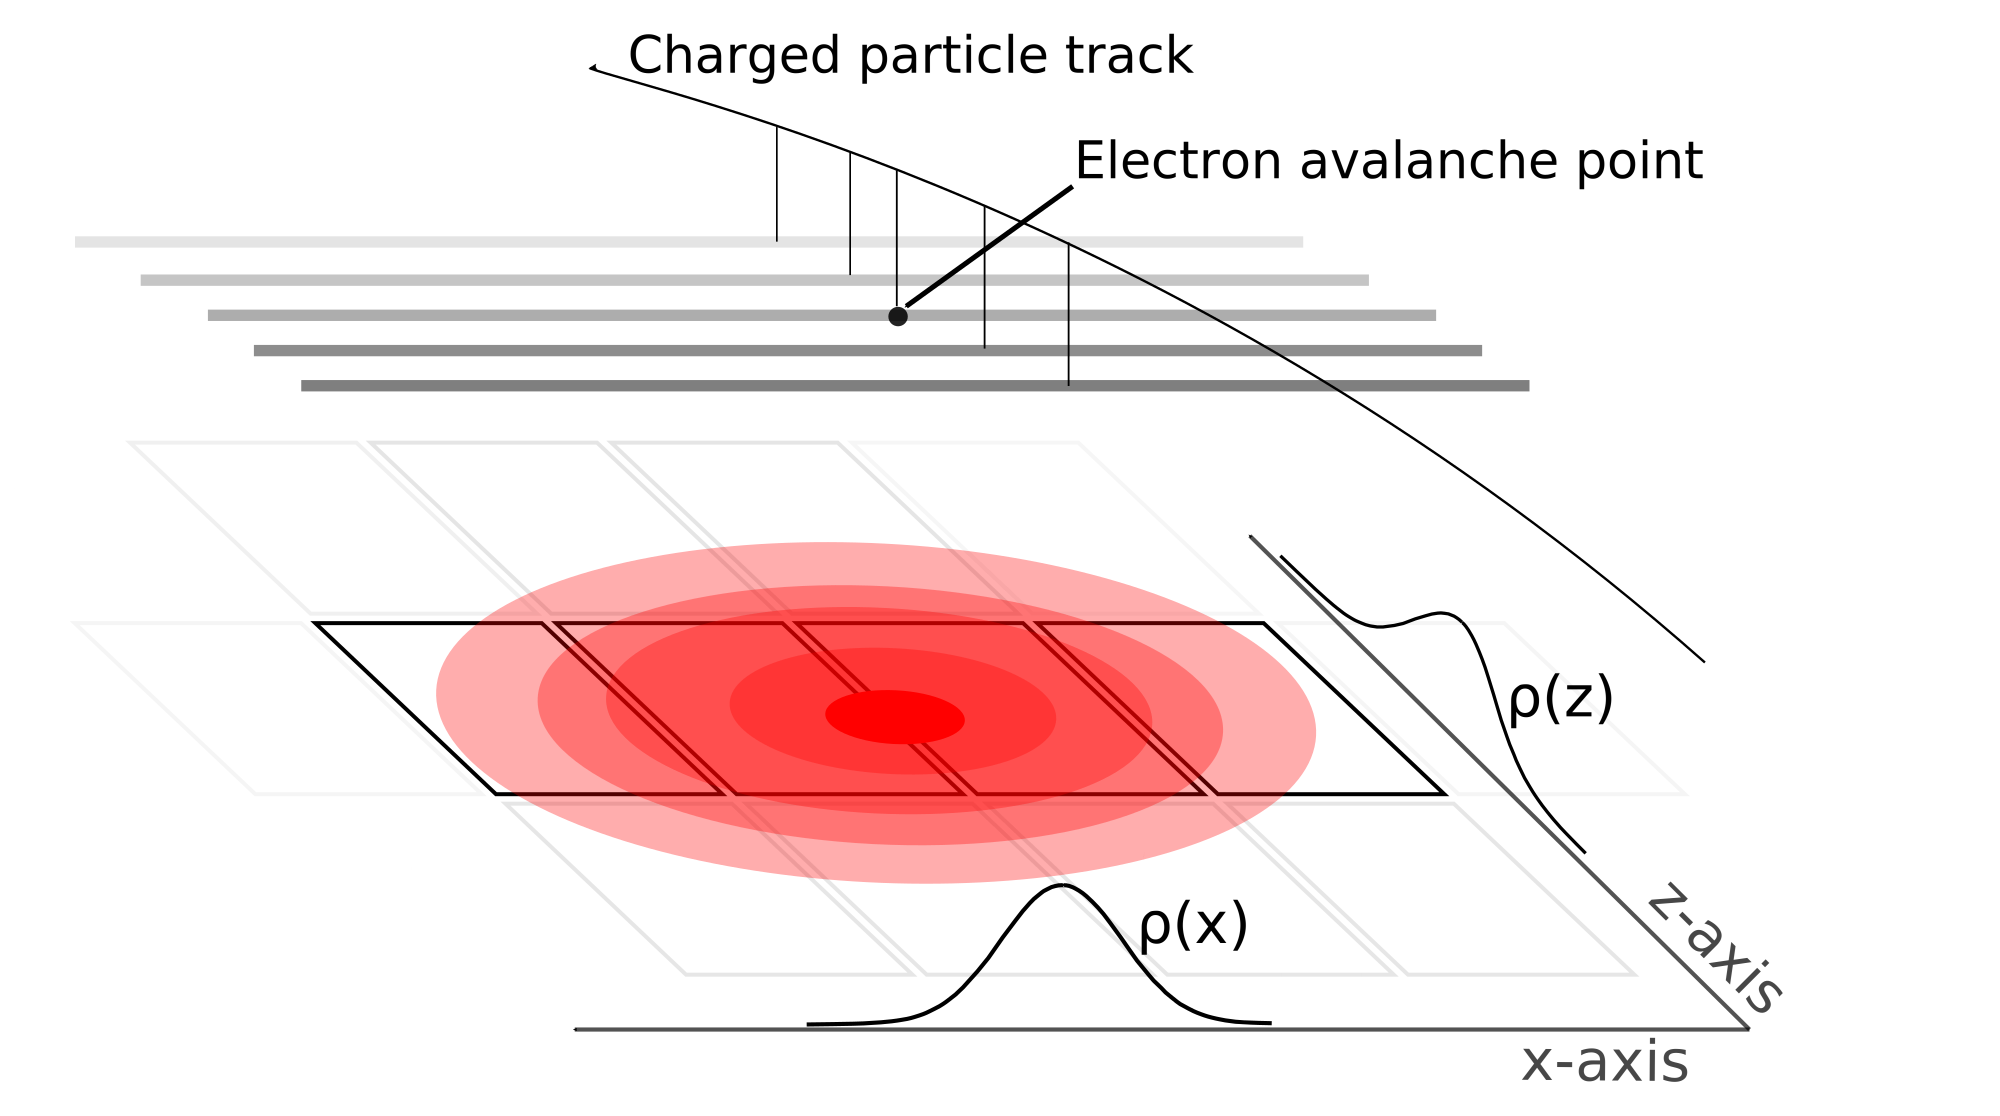
\includegraphics[width=\linewidth]{padsat_Large}
\caption{A cartoon illustration of the charge distribution resulting from an electron avalanche on one wire and the projections of the distribution onto the two axis $\rho(x)$ onto the x-axis and $\rho(z)$ onto the z-axis. The orientation of the wire planes is flipped upside down to display the perspective better.}
\label{fig:2DPRF}
\end{figure}

Gatti \cite{gatti} derived a semi-empirical formula for the charge distribution in a simple multi-wire TPC given as, 
\begin{equation}\label{eq:gatti}
\begin{split}
PRF_{\mathrm{Gatti}}(\lambda)
& = \frac{K_{1}}{K_{2}\sqrt{K_{3}}}\bigl[\arctan(\sqrt{K_{3}}\tanh\bigl[K_{2}\bigl(\frac{\lambda}{h}+\frac{w}{2h}\bigr)\bigr]) \\
& - \arctan(\sqrt{K_{3}}\tanh\bigl[K_{2}\bigl(\frac{\lambda}{h}-\frac{w}{2h}\bigr)\bigr])\bigr] \\
\end{split}
\end{equation}

where $w$ is the width of the pad, $h$ is the distance of the anode plane to the pad plane, and $\lambda$ is the distance of the pad center to the avalanche point. It is a single parameter equation where the two parameters $K_1 = \frac{K_{2}\sqrt{K_3}}{4 \arctan(\sqrt{K_3})}$ and $K_2 = \frac{\pi}{2}\left(1-\frac{\sqrt{K_{3}}}{2}\right)$ depend on the parameter $K_3$, which is a function of the ratio of the anode wire diameter to the distance of the anode wires to the pad plane. $K_3$ can be looked up in a graph in \cite{blumrol} and \cite{gatti}.



\subsection{Experimental Pad Response Function}

The correlations we introduced by only clustering along one direction do not play a significant role in the particle identification, but cause deviations from the expected Gatti distribution. Also, analytic PRFs only exist for classical multi-wire TPCs. For these reasons it is useful to experimentally measure the PRF and fit it with an empirical function, typically a Gaussian, to describe its behavior. 

As in Fig.~\ref{fig:topview}, we postulate that the PRF is a function of the total charge deposited in a cluster $Q = \sum_i q_i$, and the difference in position of the center of the $i^{th}$ pad, $x_i$, to the mean position $\bar{x} = \sum_i x_i q_i/Q$, defined as $\lambda_i = x_i-\bar{x}$. The PRF is simply defined as the charge fraction of each pad as a function of $\lambda$, as shown in Equation \ref{eq:prf}. 

\begin{equation}\label{eq:prf}
PRF(\lambda_i) = \frac{q_i(\lambda_i)}{Q}
\end{equation}

Averaging over many events in the experimental data, the resulting PRF for the S$\pi$RIT TPC is shown in Fig.~\ref{fig:expprf}. Here we see the deviations from the expected analytic Gatti distribution (black curve), whereas fitting with a two parameter Gaussian function (red curve) gives a better description of the  data, Eq.~\ref{eq:gaus}, with the two parameters being the normalization coefficient, $N_0$, width $\sigma$, and with a mean value assumed to be 0.

\begin{equation}\label{eq:gaus}
PRF_{\mathrm{Gaus}}(\lambda) = N_0 e^\frac{-\lambda^2}{2\sigma^2}
\end{equation}

\begin{figure}[ht!]s
\begin{overpic}[width=\linewidth]{fig5.pdf}
\put(61,55){\contour{white}{ PRF${}_{\mathrm{Gaus}}(\lambda)$ eq. \ref{eq:gaus}  }}
\put(61,49){\contour{white}{ PRF${}_{\mathrm{Gatti}}(\lambda)$ eq. \ref{eq:gatti} }}
\end{overpic}
\caption{Experimental pad response function of many events for a crossing angle of $85^{\circ} < \theta \leq 90^{\circ}$.  }
\label{fig:expprf}
\end{figure}

The shape of the PRF depends on the crossing angle of the track \cite{gatti}. Plotted in Fig.~\ref{fig:prfpimData} is the PRF of $\pi^-$ tracks vs. the crossing angle $\theta$. The PRF gets wider starting from $90^{\circ}$  and going to $45^{\circ}$; if we did not switch clustering directions the PRF would become wider until it was a uniform distribution and there was no position resolution. Since we switch the clustering direction from $x$ to the $z$ direction at $45^{\circ}$, the opposite trend is seen where the PRF becomes narrower as the position resolution gets better going from $45^{\circ}$ to $0^{\circ}$.




\begin{figure}[!htb]
     \centering
	 \includegraphics[width=\textwidth]{PRFs_data_wcut.png}
     \caption{PRF response from $\pi^-$ data. }
     \label{fig:prfpimData}
\end{figure}

\begin{figure}[ht!]
\vspace{5mm}
\includegraphics[width=\linewidth]{fig7}
\caption{Parameters $N_{0}$ and $\sigma$ as a function of the crossing angle $\theta$ with the $4^{th}$ order polynomial fits.}
\label{fig:normsigma}
\end{figure}

\begin{comment}
\begin{table}
\centering
 \begin{tabular}{||c c c c c c||} 
 \hline
 Coefficient & $c_0$ & $c_1$ & $c_2$ & $c_3$ & $c_4$ \\ [0.5ex] 
 \hline\hline
 $0 < \theta < 45$ & & & & &  \\ [.25ex]
 \hline
 $N_0$ & .897 & 5.766E-3 & -4.263E-4 & 7.444E-6 & 5.705E-8 \\ 
 \hline
 $\sigma$ & 5.496 & -3.920E-2 & 2.693E-3 & -5.208E-5 & 5.334E-7\\
 \hline
 $45 < \theta < 90$ & & & &  & \\ [.25ex]
 \hline	
 $N_0$ & 1.220 & -6.258E-2 & 1.608E-3 & -1.492E-5  & 4.654E-8 \\
 \hline
 $\sigma$ & 31.368 & -1.109 & 1.779E-2 & -1.336E-4 & 3.940E-7\\
 \hline
\end{tabular}
\caption{Coefficients of the $4_th$ order polynomial fit to the Gaussian parameters $N_0$ and $\sigma$. The polynomial form is given as $c_0 + c_1 x + c_2 x^2 + c_3 x^3 + c_4 x^4$}
\label{tb:coeff}
\end{table}
\end{comment}
 
Fits were performed to the experimental data with  $5^{\circ}$ width bins from $0^{\circ} < \theta \leq 90^{\circ}$. The two parameters of the Gaussian fits are plotted versus $\theta$ in Fig.~\ref{fig:normsigma}; a $4^{th}$ order polynomial fit between these points allowed for interpolating between $\theta$.


\subsection{Considerations when constructing a TPC}
Several considerations went into the construction of the S$\pi$RI TPC which I wish to summarize and document here. All materials and glues of the TPC were selected as low out-gassing materials. Several materials (that are common place in nuclear labs), such as vacuum grease, viton o-rings, all out-gas organic chemicals into the counter gas which damage the TPC by permanently lowering the gain over time. The organic molecules responsible are difficult to identify exactly, but lists of good and bad materials are well known in the literature from experiments. If a material we wished to used was not on these lists we placed the material in a clean chamber with the counter gas and flowed this counter gas through a small proportional counter making sure the gain did not drop at high collection rates when exposed to a high rate alpha Americium source. 

Sparking
Two volumes of gas. 



\section{Ancillary Detectors }


\subsection{Kyoto Multiplicity Trigger}
%kyoto array sets multiplicity trigger
%scintillator bars
The Kyoto Multiplicity Array consists of two arrays of plastic scintillating bars on each side of the TPC, each consisting of 30 bars. The entire TPC structure was designed so that light charged particles could easily pass through  the field cage and  side walls of the TPC enclosure. In this way the number of tracks passing through the sides of the TPC could be measured by this array. In heavy ion collisions the more central a nuclear collision is, the more nucleons participate in the collision, resulting in more measured tracks. It is this correlation between the number of tracks and centrality of the collision that makes the Kyoto Array sensitive to the centrality of events. It is more likely that in very central collisions more tracks are going to the peripheral angles and measured by the Kyoto array. In the experiment the trigger selection criteria was $n_{Kyoto} > 4$, where $n_{Kyoto}$ is the total number of tracks measured by both arrays. 

\begin{figure}[!htb]
\includegraphics[width=\textwidth]{TPCAux.png}
\label{fig:aux}
\caption{Exploded views of Kyoto and KATANA arrays.}
\end{figure}


\subsection{Krakow KATANA Veto and Multiplicity Array}
%beam veto
%beam trigger optional
The Krakow KATANA array consists of 12 plastic scintillating bars mounted to the downstream wall of the TPC enclosure. Three of the 12 bars were thin and operated as a beam veto in the event the beam did not make a nuclear collision with the target; this was a majority of the time. The 9 other bars operated as an additional multiplicity array similar to the Kyoto array. Since most of the particles are focus forward in a cone in the laboratory frame, it was found the condition on the Kyoto array was sufficient to trigger on central events; thus the KATANA array was used in primarily the beam veto mode. This was accomplished by positioning the array so that the expected position of the beam exiting the TPC would be centered on the three thin paddles. The threshold of the veto paddles were set so that the charge of a particle, $Z$, was $Z > 20$. This allowed the selection of very central events and we did not trigger on very peripheral or no collision events. 


\subsection{Active Veto Array}
The beam was tuned by two sets of quadropole  magnets, STQ 1 and STQ2, so that the beam spot was focused on the TPC target location. Because of the inherent angular dispersion of the beam there were incoming beam events which significantly deviated from the target location. To veto these type of events an active veto array was set at the entrance of the TPC consisting of four small scintillating bars arranged to be slightly larger than the target size. The threshold was set so that any beam particle which passed through any of the bars it would send a trigger signal to not trigger the system since the beam path would not be on target but on some other material inside the TPC. 

\section{Radio Isotope Beam Factory (RIBF) Facility }
%Cyclotron facility overview.
%Samurai line overview.
%Beam line element overview.
%Big rips beam PID. reference 
The primary and secondary beams were produced at the Radioactive Isotope Beam Factory (RIFB) facility at RIKEN, in Wako-shi, Japan. The RIBF facility starts with two primary beam types, ${}^{132}$Xe and ${}^{238}$U, which produced by an ion-source and accelerated to progressively higher kinetic energies by 1 linear accelerator (RILAC), and 4 different cyclotrons (RRC, fRC, IRC, and SRC), reaching a primary beam energy of \SI{345}{\MeVA}. 



\begin{figure}[!htb]
\includegraphics[width=\linewidth]{SAMURAI-beamline.png}
\caption{Overview of the RIBF, BigRIPS, and SAMURAI beamline.}
\label{fig:samuraiBeamLine}
\end{figure}

After the SCR, the primary beams impinge on a rotating \SI{3}{\milli\metre} Be target which produces many different species by fragmentation. These fragments are then separated by the BigRIPS spectrometer which is tuned to the particular secondary fragment of interest. This is accomplished through several dipole magnets, slits, and wedge degraders. The resulting secondary beam is not pure and the purity depends on the primary beam and target beam desired.

In these set of experiments several beams were produced with varying intensities and purities. Table~\ref{tb:beams} summarizes the average qualities of the 4 secondary beams produced in the two experimental campaigns. 

 \begin{table*}\centering
\ra{1.3}
\begin{tabular}{@{}rrrrr@{}}\toprule 
 Primary Beam & Secondary Beam & Energy at mid target \si{\MeVA} & Intensity \si{\kilo\hertz} & Purity (\%) \\ [0.5ex] 
 \midrule
 ${}^{238}$U   & ${}^{132}$Sn   &  269.2  &  9.5  &  54   \\
 ${}^{238}$U   & ${}^{124}$Sn   &  270.3  &  9.1  &  10  \\
 ${}^{124}$Xe  & ${}^{112}$Sn   &  270.4  &  7.6  &  48  \\
 ${}^{124}$Xe  & ${}^{108}$Sn   &  269.3  &  7.5  &  52   \\
 \bottomrule
\end{tabular}
\caption{Primary and secondary beam properties produced in the \spirit TPC experimental campaigns. }
\label{tb:beams}
\end{table*}



\section{Experimental Setup}

The \spirit TPC was designed to fit exactly into the dipole gap of the  dipole magnet at the end of the BigRIPS beam line. Figure~\ref{fig:experiment} shows a drawing of the \spirit TPC inside of the SAMURAI magnet chamber which was rotated to the $\ang{0}$ configuration. Typically the SAMURAI (Superconducting Analyzer for Multi-particles from Radioisotope beams) is operated under vacuum as a large-acceptance multi-particle spectrometer for radioactive-beam experiments. This magnet can reach magnetic fields up to \SI{3}{\tesla} at the center of the pole gap. The space between the magnetic pole faces is further complicated by large bolts which protrude from the pole faces. These bolts secure the vacuum chamber to the magnet which is not practically removable; though the inside of the magnet was not operated under vacuum. This required an extensive rail system and support frame to slowly slide in the TPC over the bolts, finally raising the TPC several \si{\centi\metre} to the final height. 

The height of the TPC was roughly aligned with a self-leveling laser system to match the center of target with the center of the beam line. Once the TPC was adjusted to the final location, the position of the TPC was measured in fine detail with a photogrametry system CITE HERE. Small highly reflective targets were placed all over the TPC both inside and out and pictures were taken with a calibrated lens and camera system. Using the commercial software provided the set of different camera perspectives reconstruct a point cloud of all the targets into 3-dimensional coordinates. Since the magnet was also measured with the same system after installation, we can match the two systems to get the absolute position of the TPC -- and several of its internal components-- relative to the magnet frame. The position resolution of this type of system was estimated to be around \SI{200}{\micro\metre} for each coordinate, which is much more precise than needed CITE HERE or Show data.

Maybe put a position table summary here of the TPC position and definition of the coordinates system in the TPC frame and the Magnet frame


\begin{figure}
\includegraphics[width=\textwidth]{perspective.png}
\caption{Drawing of the experimental setup with the TPC inside of the SAMURAI magnet at $\ang{0}$ configuration.}
\label{fig:experiment}
\end{figure}


\section{Data Acquisition (DAQ) }
The Data AcQuisition (DAQ) consisted of three different systems. The RIBFDAQ system served as the master DAQ for the BigRIPS beam identificaiton DAQ, the TPC DAQ, the NeuLAND neutron wall DAQ, and the Kyoto Array DAQ systems. The TPC DAQ was handled by the NARVAL framework to readout the GET electronics for the \spirit TPC. A General Trigger Operator (GTO) trigger was supplied to each DAQ synchronizing the subsystems. 

\section{Trigger Condition}
Signals from all of the auxiliary detectors were combined into several logic combinations to form a trigger logic for triggering the data acquisition  (DAQ) to record data. An upstream scintillating bar formed the start counter signal, triggering on any beam coming down the beam line. The active veto will trigger for any beam that is incident off the target location. The KATANA veto produces a signal if the beam passed through the TPC un-reacted, causing no nuclear collision; this produces a veto signal with a width of \SI{4}{\micro\second} which is the approximate time it takes for the beam to drift and clear the field cage volume. The Kyoto multiplicity trigger produces a signal when the total number of tracks passing through both Kyoto arrays are greater than 4. 


\begin{figure}[!htb]
\includegraphics[width=\linewidth]{KatanaLogic.png}
\caption{KATANA trigger box logic.}
\label{fig:katanaLogic}
\end{figure}

\begin{figure}[!htb]
\includegraphics[width=\linewidth]{TriggerLogic.png} 
\caption{Master trigger logic.}
\label{fig:trigLogic} 
\end{figure}



\begin{figure}[!htb]
    \centering
    \begin{subfigure}[t]{0.45\textwidth}
        \centering
        \includegraphics[width=\linewidth]{DataTrigger1.png} 
        \caption{${}^{124}$Xe primary beam trigger.} \label{fig:dataTrigger1}
    \end{subfigure}
    \hfill
    \begin{subfigure}[t]{0.45\textwidth}
        \centering
        \includegraphics[width=\linewidth]{DataTrigger2.png} 
        \caption{${}^{238}$U primary beam trigger.} \label{fig:dataTrigger2}
    \end{subfigure}
\label{fig:datatrigger}
\end{figure}


There were several special trigger considerations when we built the trigger for the TPC. We required that the gating grid be opened fast to not miss any signal; as soon as there was a condition satisfying the Start Counter, Kyoto Multiplicity, the DAQ was not busy, and there was not a KATANA Veto signal. This was referred to as the Fast Trigger. If the KATANA trigger box is not satisfied --described later-- this will trigger a Fast Clear signal which will not trigger the DAQ and will quickly close the gating grid. Figure~\ref{fig:trigLogic} shows the logic of both of these triggers. 

The master trigger for the DAQ was different for each primary beam as the experiment got progressively better. During the ${}^{124}$Xe primary beam, the KATANA trigger box was an input into the trigger logic where as in the ${}^{238}$U primary beam, the KATANA trigger box functioned as the trigger logic utilizing the internal trigger electronics. In either case the differences in the trigger were very minor and they both behaved practically the same except for minor details on the gating grid trigger CITE HERE JONS THESIS. Figure~\ref{fig:katanaLogic} summarizes the KATANA trigger box logic. 

Figure~\ref{fig:dataTrigger1} summarizes the ${}^{132}$Xe primary beam, where the condition to produce a true KATANA trigger output was there must be a Start Counter, KATANA multiplicity, no Veto, and no DAQ busy signal. The KATANA trigger, Kyoto Muliplicity, and Start Counter together trigger the DAQ. 

 Where as Fig.~\ref{fig:dataTrigger2} summarizes the ${}^{132}$Xe primary beam, where the condition to produce a true KATANA trigger output was there must be a Start Counter, Kyoto or KATANA multiplicity, no Veto, and no DAQ busy signal. Here the KATANA trigger and the SC SUM??? togethere trigger the DAQ. 
 
 It is worth mentioning how the busy signals for the experiment were handled. The DAQ system itself produces a busy signal which was combined with the busy signals from either opening or closing the gating grid. When opening the gating grid it is assumed the full volume of the TPC will be read out and therefore  a \SI{11}{\micro\second} gate is produced; which is slightly more than the time it takes for all the electrons to drift in the field cage. In the case were the gating grid should be fast closed, either due to the fast clear circuit or the end of the TPC measurement, a \SI{5}{\micro\second} gate is produced to allow for the gating grid to settle to a closed configuration and clear the drift volume of any residual electrons from the beam. Both of these gates are included with the DAQ in an OR configuration which makes the overall busy signal. 
 



\section{Collision Data Taken}


\chapter{Data Analysis I: Calibration and Corrections}

Need to explain pedestal subtraction 
GG noise subtraction 

\section{Software}

The S$\pi$RITROOT software is modular tasked based code based on the FAIRROOT package written in C++ \cite{fairroot}. The main tasks in the S$\pi$RITROOT software reconstruction are:
\begin{itemize}
  \item Decoder task
  \item Pulse Shape Algorithm (PSA Task)
  \item Helix Track Finding Algorithm
  \item Clustering Algorithm
  \item Track Fitting (GENFIT package)
  \item Vertex Fitting (RAVE package)
\end{itemize}

The decoder task converts the binary data file into a container class which maps the electronics channels into the corresponding pads and (x,z) coordinates. 

There may be several pulses in a pad coming from two tracks passing under the same pad separated  by arrival time. Using an expected pulse shape the PSA task fits the signal pulses within a pad, giving the arrival time of the drifted electrons from each particular track. The height of the fitted pulse is proportional to the total charge of that event, Q and the y-coordinate is calculated as $y = v\cdot t_0$ where $v$ is the drift velocity and $t_0$ the arrival time. Combining the information from these first two tasks, (x,y,z,Q), we construct what is called a "hit". 

 The Helix Track Finding Algorithm finds the collection of hits belonging to one track out of all the hits in an event. The hits within a track are then reduced into clusters. A cluster's position is the average position of the hits within a cluster, with the total charge of the cluster being the sum of the hits charges. 
 
 A tracks average position is estimated by the cluster's average position. The clusters are then fitted in the GENFIT track fitting package \cite{genfit}, giving the final momentum of the track. A final vertex of the event is fitted from all tracks using the package RAVE \cite{rave}. 

\paragraph{Definition of clustering}

A brief description of the method of clustering is illustrated in Figure \ref{fig:topview}. It is impractical to cluster in both the x and z-axis and we only cluster the hits along one axis. The three clusters at the bottom of Figure \ref{fig:topview} are clustered along the x-axis and the upper three are along the z-axis, as shown by the bolded pads for one of the clusters in each direction.

 The clustering direction depends on the angle  of the track with respects to the x-axis, defined as $\theta$. For example, a track going along the z-axis the crossing angle is defined as $90^{\circ}$, and a track going along the x-axis defined as $0^{\circ}$. In the case that the crossing angle is $45^{\circ} < \theta \leq 90^{\circ} $ the clustering direction is along the x-axis. For $0^{\circ} < \theta \leq 45^{\circ}$ it is along the z-axis. 

 The position along the clustering direction is calculated by weighting the individual hit's positions by their charges $q_i$ and getting the mean value. The other direction is set to the center of the pad. For example if we are clustering along the x-axis for a cluster, the z-position is set to the center of the pad in the z-direction and vice versa. 

Clustering in this way gives us better position resolution for calculating the position of each cluster. You could imagine if we calculated the clusters only along the x-axis for tracks with $\theta \approx 0^{\circ}$ the x-position is not well defined. By clustering in the direction most perpendicular to the track, we get a better position resolution.

\begin{figure}[H]
\includegraphics[scale=.5]{top_view_helix_ext.pdf}
\caption{Cartoon graphic of a top down view of a fit to a track passing through several pads. The bolded pads and the charges $q_i$ represent the hits belonging to that pad and the clusters of the track representing the average position of the track. The three clusters at the bottom are clustered in the x-direction and for the upper three clustered in the z-direction. The estimate of the position of the avalanche is given by the track fit and the position from the center to each pad to the $\bar{x}$ position is given as $\lambda_i$.}
\label{fig:topview}
\end{figure}




\section{Calibrations and Corrections}


\subsection{Cocktail calibration}

\begin{table*}\centering
\ra{1.3}
\begin{tabular}{@{}rrrrrrr@{}}\toprule
& \multicolumn{3}{c}{$100 MeV Target$}\\
\cmidrule{2-4}
Particle &\phantom{abc} & Measured & Corrected & \% Difference & \% Difference\\
\midrule
p   & 882.8 & 929.5 & 877.3   &  3.7  & -1.0  \\
d   & 817.1 & 831.15 & 797.94 &  1.7  & -2.3\\
\bottomrule
\end{tabular}
\caption{Summary of expected cocktail. }
\label{tb:cocktail100tar}
\end{table*}

\begin{table*}\centering
\ra{1.3}
\begin{tabular}{@{}rrrrrrr@{}}\toprule
& \multicolumn{3}{c}{$100 MeV$}\\
\cmidrule{2-4}
Particle & Expected & Measured & Corrected & \% Difference & \% Difference\\
\midrule
p   & 882.8 & 903.5 & 889   &  2.0   & -1.6  \\
d   & 817.1 & 898.5 & 874.5 &  2.1   & -2.7\\
\bottomrule
\end{tabular}
\caption{Summary of expected cocktail. }
\label{tb:cocktail100}
\end{table*}

\begin{table*}\centering
\ra{1.3}
\begin{tabular}{@{}rrrrrrr@{}}\toprule
& \multicolumn{3}{c}{$300 MeV$}\\
\cmidrule{2-4}
Particle & Expected & Measured & Corrected & \% Difference Raw & \% Difference Corrected\\
\midrule
d   & 1621 & 1704 & 1612   &  5.1 & -0.6  \\
t   & 1612 & 1691 & 1596   &  4.9  & -1.0\\
${}^{4}$He   & 1613 & 1698 &  5.3 & 1595  & -1.1\\

\bottomrule
\end{tabular}
\caption{Summary of expected cocktail. }
\label{tb:cocktail300}
\end{table*}


\begin{table*}\centering
\ra{1.3}
\begin{tabular}{@{}rrrrcrrrcrrr@{}}\toprule
& \multicolumn{3}{c}{$100 MeV$} & \multicolumn{3}{c}{$100 MeV$} & \multicolumn{3}{c}{$300 MeV$}\\
\cmidrule{2-4} \cmidrule{6-8} \cmidrule{10-12}
& &\multicolumn{2}{c}{Measured} & & \multicolumn{2}{c}{Measured} & & \multicolumn{2}{c}{Measured}\\
\cmidrule{3-4} \cmidrule{7-8} \cmidrule{11-12}
Particle &\phantom{abc} & Measured & E$\times$B\\
\midrule
p   & 882.8 & 929.5 & 877.3 & 903.5 & 929.5 & 889 &\phantom{abcdef} & f & f \\
d   & 817.1 & 831.15 & d & 898.5 & e & e & 1621.1 & 1704 & 1612\\
t   & 589.5 & d & d & 887 & e & e & 1612.4 & f & f  \\
$^{3}$He  & 1617.3  & d & d & 1795.2 & e & e & 3236.4 & f & f\\
$^{4}$He  & 1405.6  & d & d & 1782.9 & e & e & 3226.4 & f & f \\
\bottomrule
\end{tabular}
\caption{Summary of expected cocktail. }
\label{tb:cocktailsummary}
\end{table*}

Light charged particles (p,d,t,${}^{3}$He,${}^{4}$He), beams were produced and measured in the TPC. The magnetic and slit settings of the dipoles in the BIGRIPS spectrometer was set so that the measured momentum resolution of the beam was $\frac{\delta p}{p}$ < 1\%. Two magnetic rigidity settings were studied, with an empty target. A thick Aluminum target was used to provide a slightly lower point for part of the lower rigidity setting, effectively creating three calibration points over several particle species. The production of certain particles (t,${}^{3}$He), produced too few counts to make a good measurement, and in the high momentum rigidity setting protons could not propagate down the line and there were no counts. 

Since the expected momentum resolution resulting from the spectrometer was less than 1\%, the observed momentum resolution measured by the TPC is a good measurement of the combined momentum resolution of the software and TPC (intrinsic detection) system. The momentum resolution of the TPC depends on several factors such as the particle's angle, momentum, charge, track multiplicity, etc. This calibration beam represents and ideal situation where the track was parallel to the pad plane and only one particle was measured at one time. The energy loss resolution can also be directly inferred from the measurement since each energy setting represents a monochromatic source of each particle species, which has a well defined energy loss distribution. An average momentum resolution of ~2\% and the energy loss resolution of ~ 5\% was measured for particles ranging from protons to ${}^{4}$He, over the range of momenta measured in the calibration beam as summarized in Table~\ref{tb:momresolution}.

Since magnetic dipole setting of the BIGRIPS spectrometer define the energy of each particle type we can calculate the expected momenta of each particle species measured. Small corrections to the momenta were propagated using LISE++ software which can calculate the energy loss through several materials in the beam line. These corrections resulted in a small change in the momenta. The measured momenta of the calibration beam differed significantly from the expected values as seen in Tables~\cref{tb:cocktail100tar,tb:cocktail100,tb:cocktail300}. This effect is attributed to inhomogenatities in the magnetic field which introduces electron drift velocity in the direction of $\vec{E}\times\vec{B}$ direction. The $\vec{E}\times\vec{B}$ dift velocity causes the electron trajectories to shift toward the +x-axis in the TPC coordinates causing particles of positive charge (going in the -x-axis) to have a higher measured momenta than in reality. The disagreement in measured and expected momenta is upwards of ~5\% difference in the higher momentum calibration settings. The details of the correction technique are discussed in the later Section~\ref{sec:spacecharge} are discussed in a more general correction which also includes correction for the space charge; the same correction technique was applied here in the special case of zero space charge which is the special case of only having $\vec{E}\times\vec{B}$ components .

The values under the corrected column of seen in Tables~\cref{tb:cocktail100tar,tb:cocktail100,tb:cocktail300}, represent the data correcting for $\vec{E}\times\vec{B}$. A significant improvement is seen in the high momentum setting going from around ~5\% disagreement to within ~1\% agreement in the corrected data. For the lower momentum settings (Tables~\cref{tb:cocktail100tar,tb:cocktail100}), protons see a slight improvement of about ~1\% where as the deuterons are over corrected in both settings. The level of agreement of the all corrected values is still within the estimated momentum resolution of the TPC. 

\begin{table*}\centering
\ra{1.3}
\begin{tabular}{@{}rr@{}}\toprule
Momentum Resolution \% & <dE/dx> Resolution \% \\
\midrule
1.6  & 4.6\\
\bottomrule
\end{tabular}
\caption{Summary of expected cocktail. }
\label{tb:momresolution}
\end{table*}

Picture of cocktail before and after ExB effect
Table of LISE++ expected cocktail energies ridigity setting of dipole magnets (reference big rips line)



\subsection{Electronics calibration}
The channel number of the electronics was calibrated by measuring the response of each channel to an input pulse supplied by a pulse generator. The pulse was injected into the ground plane of the TPC. This distributed the pulse evenly across the entire pad plane over a range of input voltages. The input voltage is plotted as a function of the measured ADC channel in Fig.~\ref{fig:gaincalib} for every channel. The small variation in each channel can be seen as the wide band around each measurement point. A linear fit is performed to get the best fit line which provides a reference line which each channel is calibrated to. The right panel shows the resulting distribution of channels after calibration. This is a relative calibration technique meant to calibrate the varying gains in each channel relative to one another. 

\begin{figure}[H]
\includegraphics[width=\linewidth]{gaincalib.png}
\caption{Calibration of electronics}
\label{fig:gaincalib}
\end{figure}

\subsection{Anode gain calibration}

As mentioned earlier, the anode wires were separated into 14 independently biased sections. The high voltage of sections 12 and 14 were reduced during the experiment due to high currents being observed on the wires. The wire section voltages were lowered once and adjusted once again. Out of all the runs used in the analysis in this thesis \ref{tb:runList}, the anode sections 12 and 14 were lowered to \SI{1085}{\volt} for runs 2272-2371 and set to \SI{1214}{\volt} for all the other runs. By lowering the voltage on these anode wires, the gas gain is lowered as compared with all the other anode wire plane sections which operate at \SI{1460}{\volt}. To account for the drop in gain, in the software we increase the gain of the pads which lie above these anode wires. To calibrate these sections we perform a relative calibration to the high gain anode sections by comparing the energy loss values of the high and low gain sections. 


\begin{figure}[H]
\includegraphics[width=\linewidth]{highlowcal.png}
\caption{Calibration of low high.}
\label{fig:highlowcal}
\end{figure}


\subsection{Extending the dynamic range of the Electronics}
Using a TPC for measurements of HIC in nuclear physics presents a different set of challenges as opposed to higher energy experiments. Typically in higher energy experiments the charge of particles is Z$e$, where Z=1. Also the particles are traveling at higher energies in which the energy losses in a detector range from the minimum of the energy loss curve to the small logarithmic climb CITE FIGURE HERE!!!. The dynamic range of electronics in such experiments can cover a wide range of particle energies in the energy loss curve. In nuclear HICs, we are interested in cluster of nucleons typically from Z=1-3 resulting from the collision, and even higher in some applications. As seen in Eq.~\ref{eq:bb}, the energy loss is proportional to $Z^2$; the energy values of the resulting particles are at much lower energies which are in the $1/\beta^2$ region. The energy range and particle types covered by the electronics are significantly limited as they quickly reach the dynamic range limitations of the electronics as the charge of a particle increases and the velocity decreases. 

Several TPCs have tried to address this issue by having regions of low and high gain, either in amplification gain or in electronics gain. Here we run into the issue that high velocity particles will have little to no signal in the low gain regions. At lower velocities, particles will deposit much charge over the low gain regions but will saturate the high gain regions, whose charge values are usually lost. Only within the dynamic range will tracks have the best momentum resolution, outside the dynamic range clusters will be missing in the sections which depend on the track velocity, lowering the momentum resolution of tracking. There are ongoing efforts in the nuclear community to develop new electronics which hope to mitigate these persistent issues in TPC electronics CITE HERE, by being able to switch to a lower gain value when the maximum range is reached. Though, it is quite useful to develop a software technique which may extend the dynamic range of TPC electronics without the use of external hardware, espeically in experiments which have already been performed with older electronics technologies. 

In TPCs, the effective dynamic range can be very different from the single pad dynamic range. Typically TPCs are operated inside of a magnetic field for reconstructing momentum of each particle, which requires sub-millimeter precision in the position determination of the track path. This is achieved by averaging the charge distribution over several pads which is discussed in Section CITE HERE. Therefore the effective dynamic range is related to the relative charge values of adjacent pads (between the center pad and outside pads). For example, to measure minimum ionizing particles the signal to noise ratio of the pad with the smallest charge in the distribution should be some reasonable value, say at least 6:1. From Section CITE HERE we know the central pad in the cluster holds 80\% of the total charge, where as the two adjacent pads each hold the remaining 10\%. If we require the adjacent pads to have a signal-to-noise ratio of 6:1, then the central pad would have a signal to noise ratio of 50:1. Considering this is the signal-to-noise ratio for minimum ionizing particles, and the maximum signal-to-noise ratio is 800:1, this means the effective dynamic range in the TPC is roughly 16 times that of minimum ionizing particles. The dashed lines and vertical blue bar in Fig.~ \ref{fig:intro} are separated by a factor of 20, representing the typical effective dynamic range in a TPC. This dynamic range estimate should be regarded as approximate because the energy loss fluctuates significantly about the most probable energy loss, with a long ``Landau'' like tail, as described by Bichsel \cite{bichsel}. Nevertheless, the blue dashed lines and vertical blue bar illustrate that the range of energy losses sampled in a fixed gain readout system is limited. One can change the gain and shift the energy loss range that can be sampled, but the dynamic range itself cannot be increased.

  
\begin{figure}[ht!]
\includegraphics[width=\linewidth]{intrographic}
%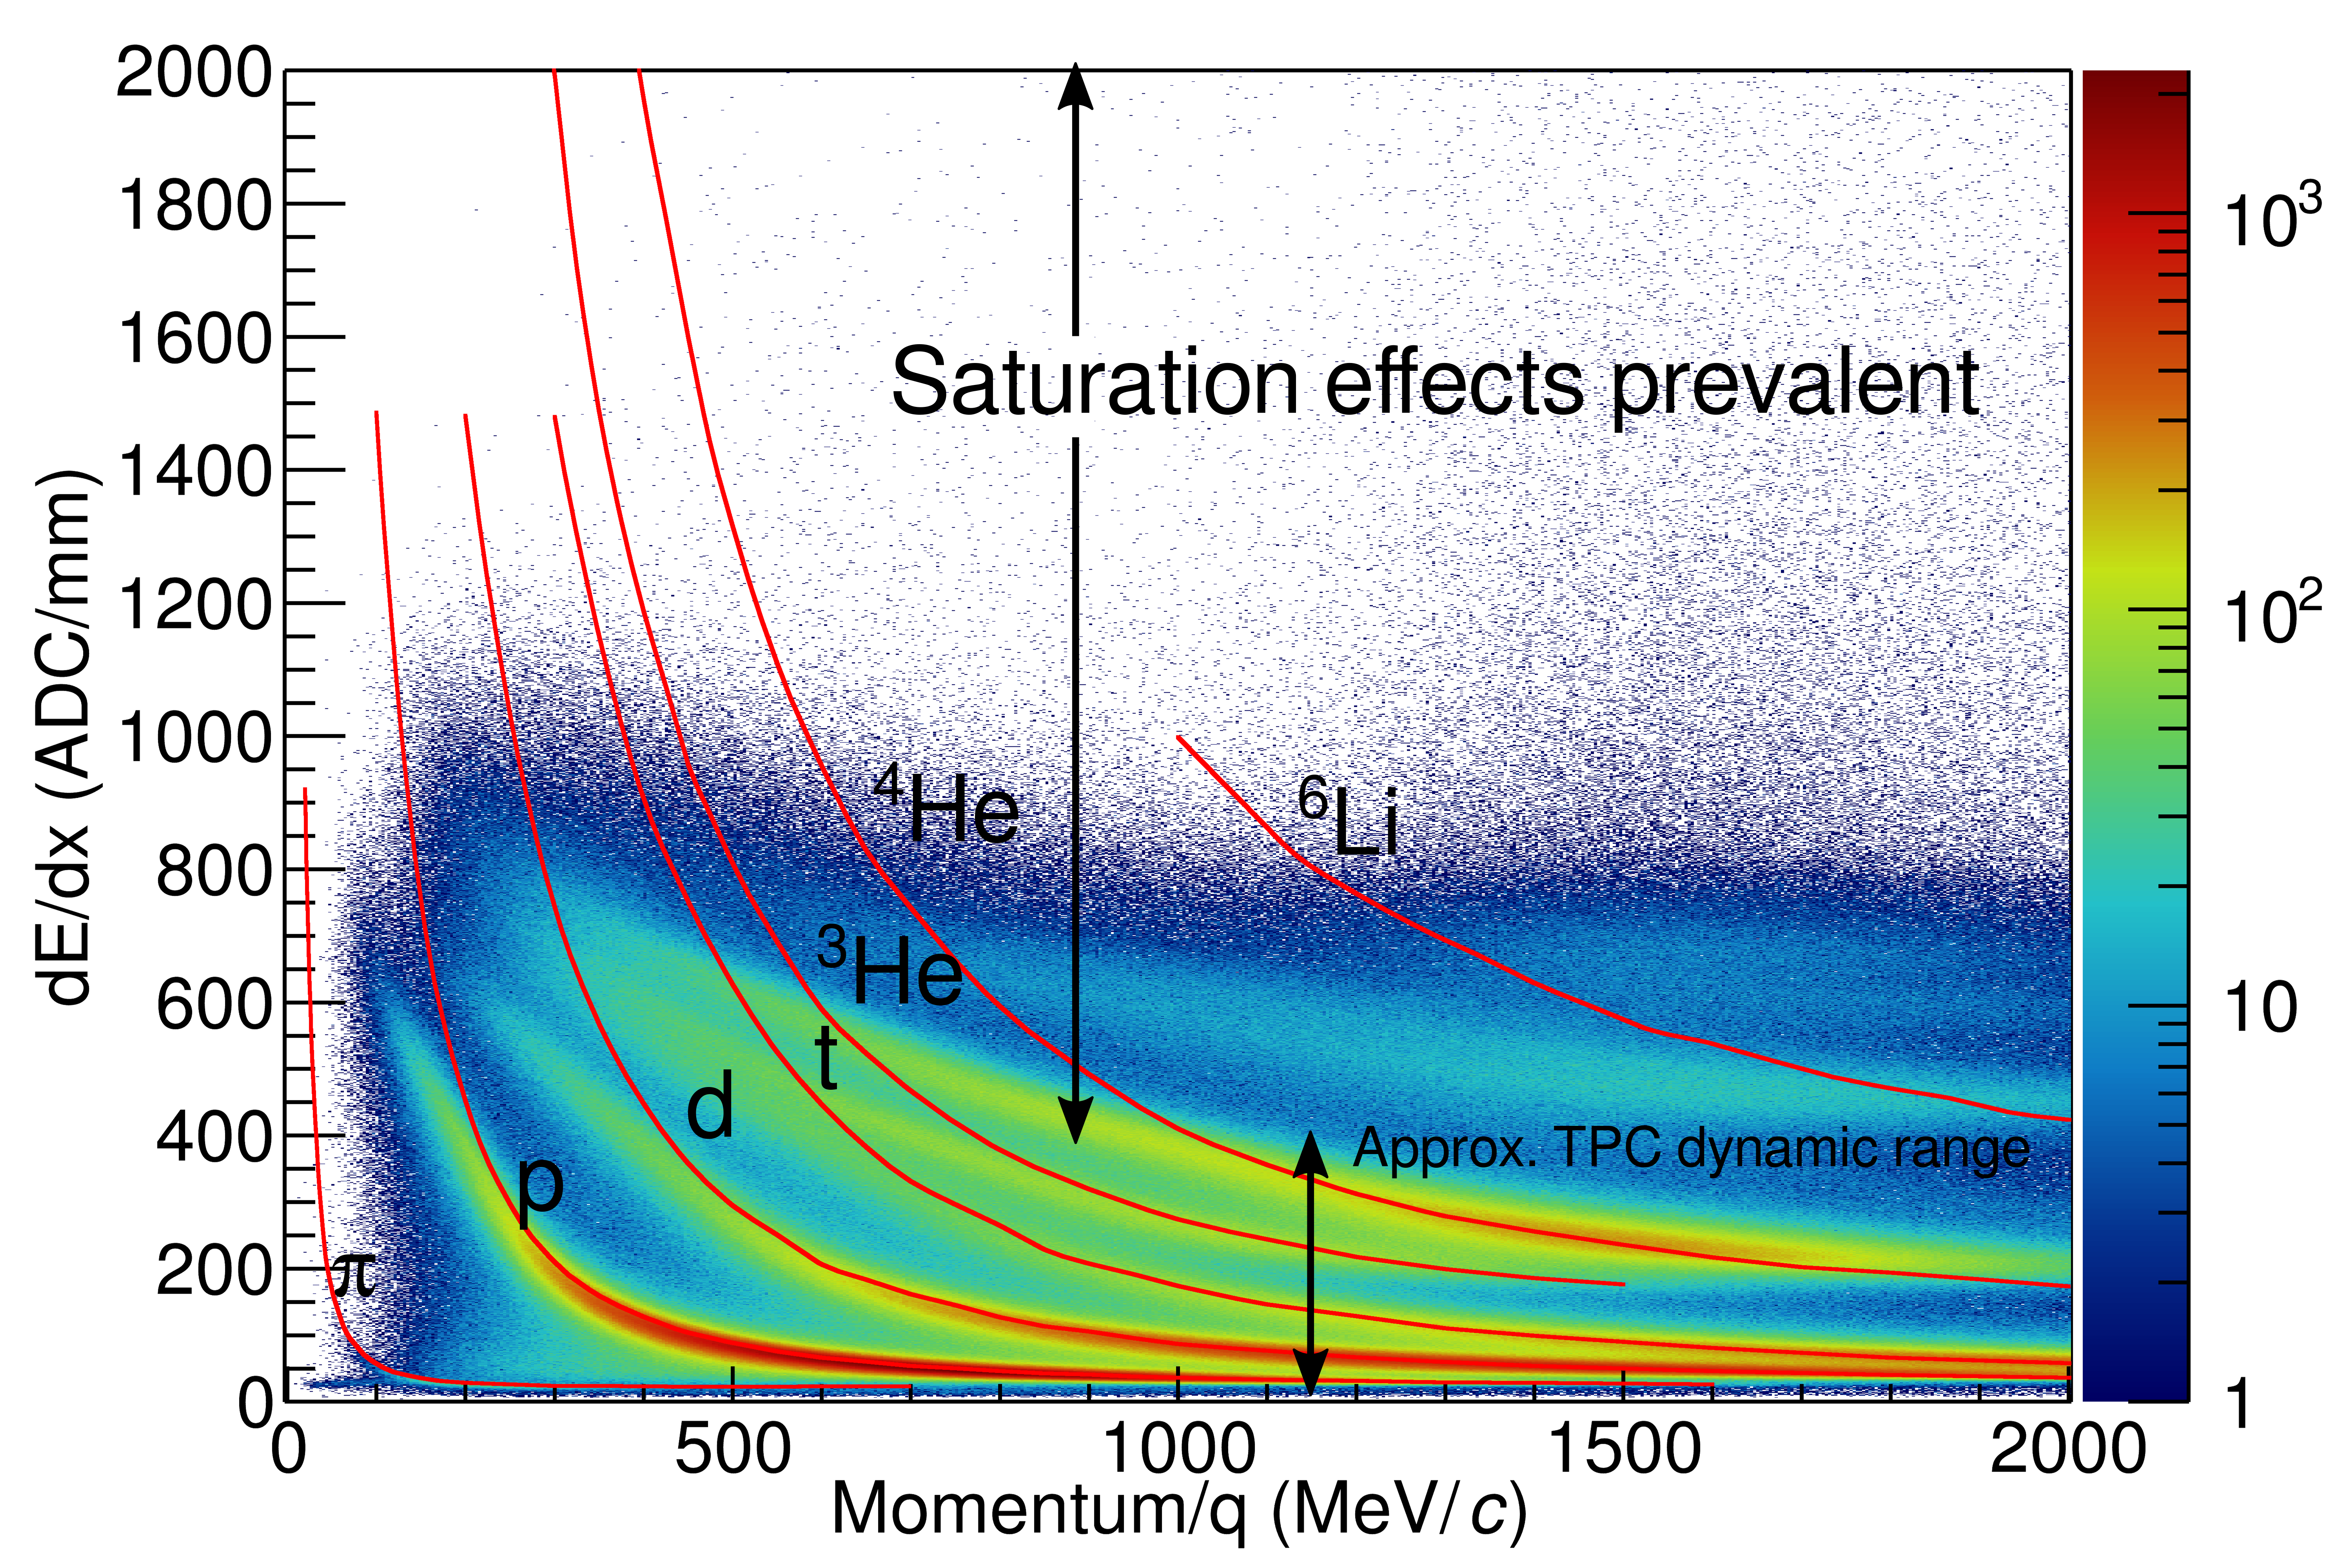
\includegraphics[width=\linewidth]{intrographic_2}
\caption{The expected $dE/dx$ lines of different particles are given in red as calculated by Geant4. The approximate dynamic range of the TPC is shown by the vertical bar for the gain setting used in the experiment. Anything outside of this region would be saturated to some degree.}
\label{fig:intro}
\end{figure}

The rapid increase in the stopping powers at low momentum illustrates the degree to which the effective dynamic range can be exceeded and highlights the problems encountered in studies of intermediate HICs, in which light particles with low momenta are abundantly produced along with highly charged particles. Similar problems are encountered when TPCs are used as active targets in direct reaction studies with rare isotope beams \cite{pattpc}. 

Several techniques have been employed to increase the observable range of energy losses. This can be done by lowering the electronics gain of selected readout channels, or by changing the gas amplification at the readout plane in certain areas of the TPC. In the EOS TPC \cite{eos} this was done by decreasing the voltages in select anode wires in the multi-wire readout. With the prototype Active Target TPC lowering or increasing the gain was achieved by decreasing or increasing the electric fields on selected pads within a Micromegas \cite{pattpc}. The results of changing the gas-gain, or the electronics gain, are rather similar in that reducing the gain to sample a range of higher energy loss makes the TPC effectively blind to minimum ionizing particles in  the regions of lower gain.



%DOUBLY DEFINED? IS THIS SUPPOSED TO BE HERE
%\begin{figure}[ht!]
%\includegraphics[scale=.5]{top_view_helix_ext.pdf}
%\caption{Cartoon of a top down view of a fit to a track passing through several pads. The bolded pads and the charges $q_i$ represent the hits belonging to that pad and the clusters of the track representing the average position of the track. The three clusters at the bottom are clustered in the $x$-direction for the upper three are clustered in the $z$-direction. The estimated position of the avalanche is given by the track fit, and the position from the center to each pad to the $\bar{x}$ position is given as $\lambda_i$.}
%\label{fig:topview}
%\end{figure}

We define the clustering direction depending on the angle of the track, at the point of each cluster, with respects to the $x$ axis, defined as $\theta$. For example, the crossing angle is defined as $90^{\circ}$ for a track going along the $z$ axis, and $0^{\circ}$ for a track going along the $x$ axis. In the case that the crossing angle is $45^{\circ} < \theta \leq 90^{\circ} $ the clustering direction is along the $x$ axis. For $0^{\circ} < \theta \leq 45^{\circ}$ it is along the $z$ axis. 

 The position along the clustering direction is calculated by weighting the individual hit's positions by their charges $q_i$ and getting the mean value. The other direction is set to the center of the pad. For example, if we are clustering along the $x$ axis for a cluster, the $z$-position is set to the center of the pad in the $z$-direction and vice versa. 
 


\subsection{Method of Desaturation}
We will use the term ``desaturation'' for our process of correcting the charge values of the saturated pads. Figure \ref{fig:satpad} shows a typical situation of saturated signals. When an avalanche causes a large induced signal, the pads directly underneath collect the largest charge becoming saturated, denoted as $q_{2'}$ and $q_{3'}$. Pads further away experience smaller, non saturating charges, denoted as $q_{1}$ and $q_{4}$. Though we do not know the saturated charge values, the distribution of all charges must follow the PRF which we have experimentally measured. From the clusters crossing angle, we can get the corresponding parameters for the PRF as described above and in Fig.~\ref{fig:normsigma}.

We assume the distance of each pad to the track, $\lambda_i$, is fixed, defining the fraction of charge each pad receives as given by the $PRF(\lambda_i)$ function. 


\begin{equation}\label{eq:chi}
\chi^2 = \sum_i \frac{(q_i^{\mathrm{obs}} - q_i^{\mathrm{expect}})^2}{q_i^{\mathrm{expect}}}
\end{equation}

To determine the best estimate for the charge values of each saturated pad, a chi squared function is minimized, given in  Equation \ref{eq:chi}, where $q_i^{\mathrm{obs}}$ are the observed, non-saturated charges $q_{1}$ and $q_{4}$, and $q_i^{\mathrm{expect}}$ are the charges we expect to observe, calculated as $q_i^{\mathrm{expected}} = Q\cdot PRF(\lambda_i)$. The charges $q_{2'}$ and $q_{3'}$, make up the unknown variable and are allowed to vary in the $\chi^2$ minimization, where they are added to make up the total expected charge $Q$.


\begin{figure}[ht!]
\includegraphics[width=\linewidth]{saturated_pads}
\caption{A typical case of a saturating event. The red pulses represent the time bucket signal for each collected charge. The pads directly underneath the avalanche point, $q_{2'}$ and $q_{3'}$, are saturated while pads farther away, $q_1$ and $q_4$ are not saturated.}
\label{fig:satpad}
\end{figure}

Shown in Fig.~\ref{fig:cocktail} is a typical cocktail event, where one particle enters the TPC volume at a time and parallel to the pad plane, representing an ideal case for momentum and $dE/dx$ determination; as it does not suffer from inefficiencies of high multiplicity events seen in the collision experimental data.  

\begin{figure}[ht!]
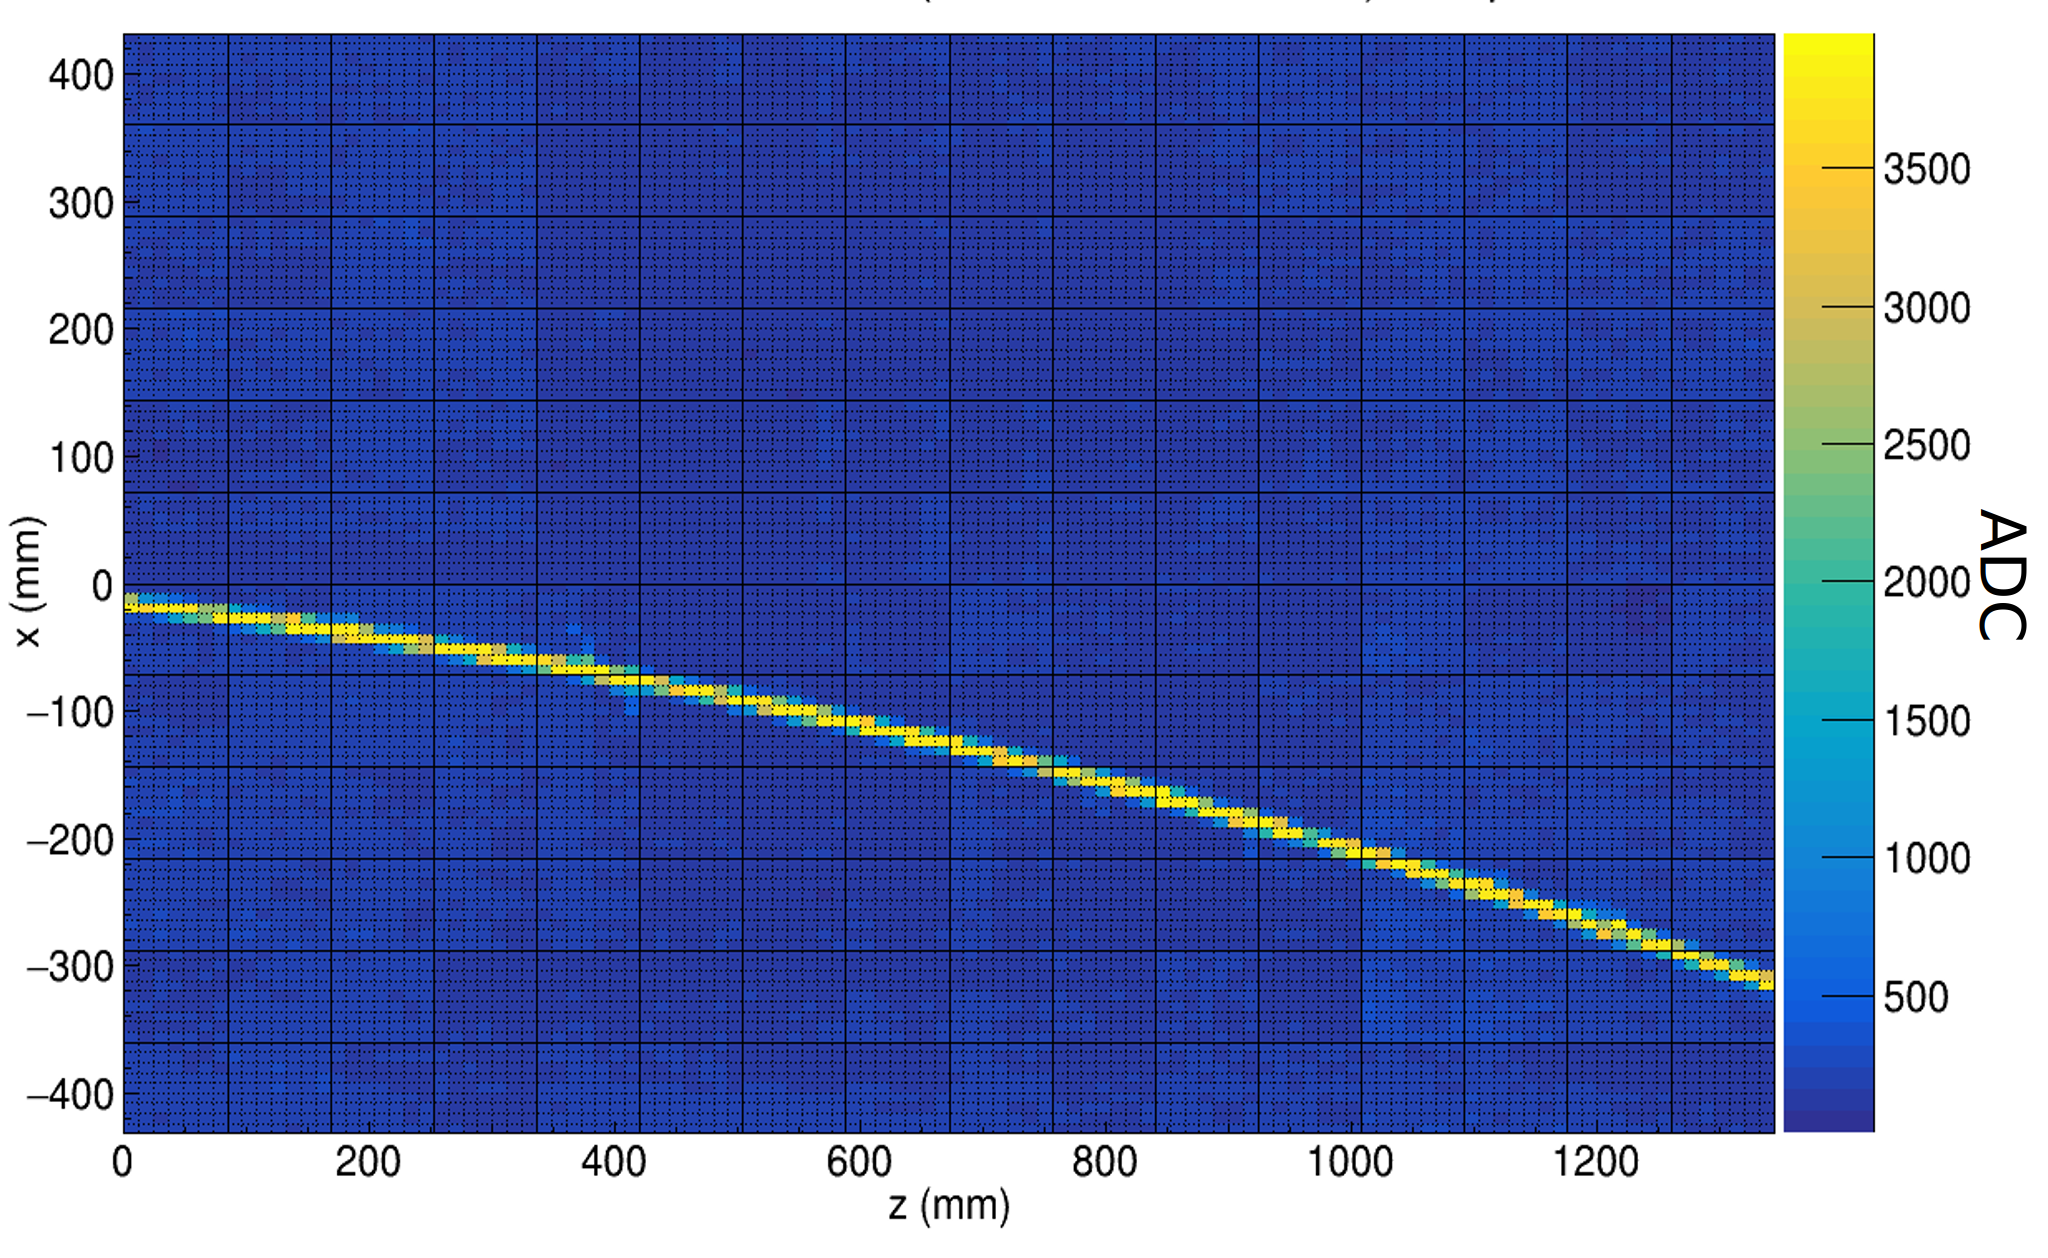
\includegraphics[width=\linewidth]{cocktail.png}
\caption{Pad plane projection for a cocktail event in the TPC.}
\label{fig:cocktail}
\end{figure}

\begin{figure}[ht!]
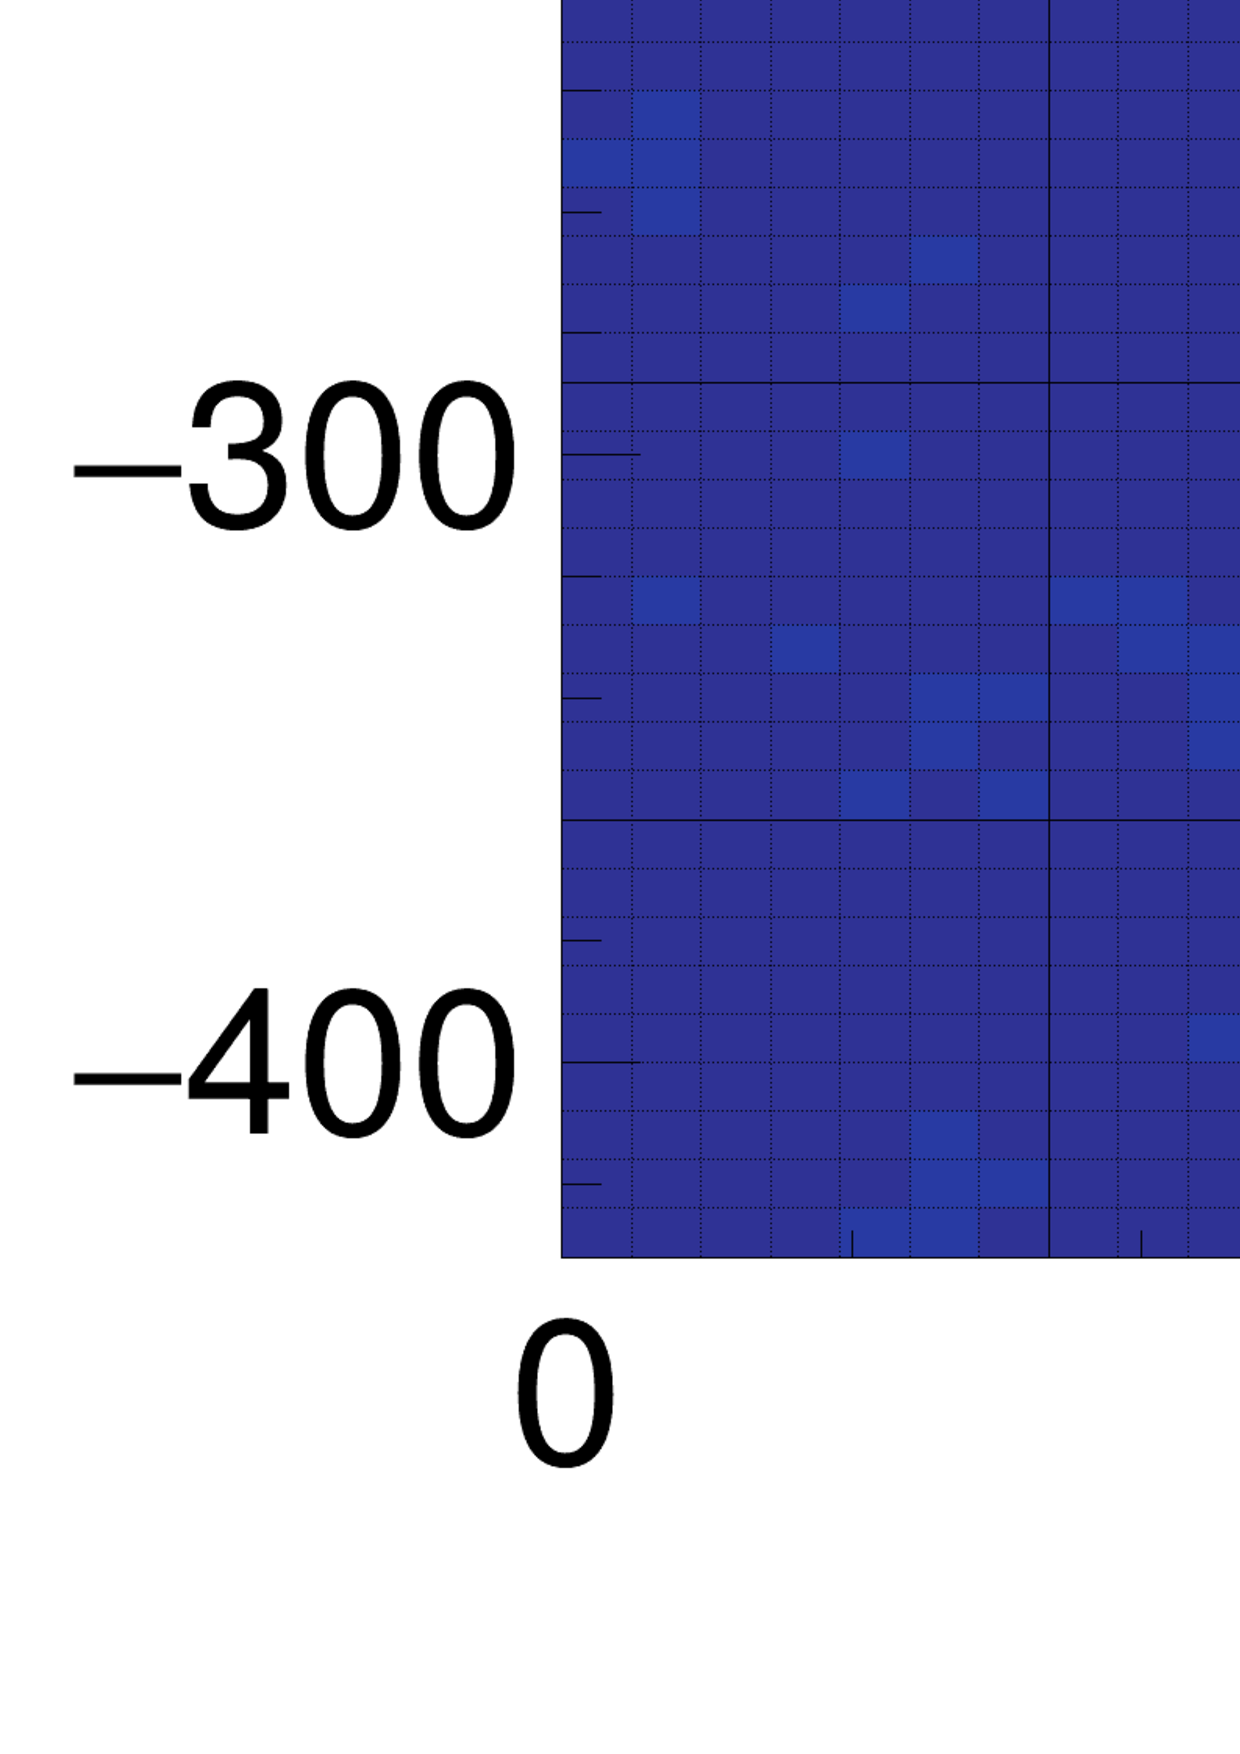
\includegraphics[width=\linewidth]{data.png}
\caption{Pad plane projection for a collision event in the TPC. Highlighted by red arrows are two regions of anode wires which had a reduced voltage of 1214 V. The voltage of the rest of the TPC anode wires are 1460 V. The reduction in voltage reduces the gain by a factor of about 10. }
\label{fig:data}
\end{figure}


\begin{figure*}[t]
\centering
\includegraphics[width=\linewidth]{dedx_compare}
\caption{The left panel shows the high gain stopping power vs low gain when the method of desaturation was not applied. In the right panel the desaturation technique was applied to the high gain region. The low gain does not suffer from saturation and represents the true $dE/dx$ value.}
\label{fig:lowvshigh}
\end{figure*}

\begin{figure*}[t]
\includegraphics[width=\linewidth]{cocktail_combine.png}
\caption{Uncorrected (left panel) and desaturated (right panel) cocktail data.}
\label{fig:cocktail_combine}
\end{figure*}

\begin{figure*}[t]
\includegraphics[width=\linewidth]{data_combine}
\caption{Uncorrected (left panel) and desaturated (right panel) collision data at polar angles of $\theta < 40^{\circ}$ and azimuthal angles between $-80^{\circ} < \phi < 80^{\circ}$}
\label{fig:data_combine}
\end{figure*}

Tracks which saturate pads in the high gain region are not saturated in the low gain region. By comparing the dE/dx values of these two sections, we can directly measure the success of the desaturation in the high gain regions using the method described above.  
 
In Fig.~\ref{fig:lowvshigh}, the effect of saturation can be seen in the high gain region for the uncorrected data. For signals below 400 ADC/mm \footnote{Un-calibrated ADC channels in arbitrary units.} the electronics are not saturated, and therefore the high and low gain sections agree. The data starts to saturate above 400 ADC/mm in the high gain channels eventually reaching a plateau while the low gain sections are not saturated and provide the true $dE/dx$ values.
 After applying the desaturation method, the correlation between the high and low gain sections is restored, as seen in Fig.~\ref{fig:lowvshigh}. From this comparison, we infer that the correction works up to signals of 2000 ADC/mm, increasing the dynamic range by a factor of at least 5.


Comparing the low to high gain sections directly validates the desaturation technique, but the goal  of this exercise is to improve the particle identification (PID). In the following PID plots the red lines represent the most probable energy loss as given by Geant4 straggling functions. A linear calibration was performed to convert keV in Geant4 to ADC in the experiment given by $ADC/mm = 19\;keV/cm$.

There are pronounced PID lines of several particle species in both the uncorrected and corrected cocktail beam PID shown in the subplots of Fig.~\ref{fig:cocktail_combine}. Three ovals around a momentum of 1700~MeV/$c$/q and two near 900~MeV/$c$/q correspond to the three $B\rho$ settings injected into the TPC. The tails of the PID lines are resulting from the particles passing through the walls and other materials outside the main detector volume, therefore lowering the initial momentum. 

The uncorrected data in Fig.~\ref{fig:cocktail_combine} shows the effects of saturation; the PID lines deviate from their theoretical expectations starting at around 400~ADC/mm eventually reaching a plateau. After applying the desaturation technique, we see a large improvement, most notably for the He and Li particles, which suffer the most from saturation. A more subtle improvement of the lighter particles, (p, d, t), can also be seen in the PID lines at lower momenta.

Looking at the collision data, shown in Fig.~\ref{fig:data_combine}, we also see a similar result. In the collision data, the PID suffers from more background and inefficiencies than the cocktail beam, nevertheless we can see a similar improvement in the PID lines when comparing before and after applying desaturation. Notably the largest improvement is the separation of particle species at lower momenta and the separation of the Li species into ${}^{6}$Li and ${}^{7}$Li. In these regions, there was little to no PID resolution before desaturation. 

The dynamic range was extended by at least a factor of 5, as demonstrated by the improved PID lines, and quantified by direct comparison to low gain sections of the TPC. This improved PID will allow for us to extend the momentum distributions of all species to lower momenta and to heavier ions than what was previously available. 


\subsection{Space Charge Corrections}
\label{sec:spacecharge}

MAYBE ADD A LITTLE NAPKIN CALCULATION OF SPACE CHARGE TO SHOW ORDER OF EFFECT. 

\begin{table}[!htp] % not just 'h!'
\centering % not a center environment
\begin{tabular}{
  @{}
  l
  S[table-format=1.2]
  S[table-format=1.2]
  S[table-format=1.2]
  S[table-format=5.2]
  S[table-format=5.2]
  @{}
}
\toprule
Beam Energy Loss  &
 {${}^{132}$Sn} &
 {${}^{124}$Sn} &
 {${}^{112}$Sn} &
 {${}^{108}$Sn} &
  {Avg.}\\
  
\midrule
$\si{\kilo\eV\per\centi\meter}$ & 11.2   &.034  &5.43   &  903   &150     \\
\bottomrule
\end{tabular}

\caption{Average energy loss of each beam.}
\label{tb:beameloss}
\end{table}

\begin{figure}[H]
\includegraphics[width=\linewidth]{spacechg_cartoon.png}
\caption{Location of space charge in 132 Sn}
\label{fig:spacechg_cartoon}
\end{figure}


\begin{figure}[H]
\includegraphics[width=\linewidth]{beampath.png}
\caption{Beam path of the experiments}
\label{fig:beampaths}
\end{figure}


As the beam passes through the field cage it ionizes the gas along the way creating electron-ion pairs. The drift velocities of the ions are \num{1e4} times slower than the electron drift velocities. Because ions move very slow, the potential build up of positive ions may create a space charge which distorts the drifting electrons of the tracks, impacting the measurement of their momentum. There are several regions of the TPC in which electron-ion pairs are created. The largest source of positive ions are created in the avalanche process near the anode wires. These ions slowly drift toward the cathode and are captured by the gating grid. The other source of ions come from the primary ionization produced by the beam and reaction products in the detector gas. The energy loss <dE/dx>$\propto Z^2$, where Z is the charge of the particle type. Because the charge of the un-reacted beam is around Z~50, the ionization due to the beam is a factor of \num{2.5e3} times that of the light charged particles which mostly are of charge Z~1. 
 The beam is positioned about 25\si{\centi\metre} below the anode plane in the TPC. It takes electrons approximately 5\si{\micro\sec} to drift to the anode plane. It takes the ions \num{5e4}\si{\micro\sec} to travel. The beam rate in the experiment varied around a value of about 10\si{\kilo\hertz}, which has an average occurrence of 1 beam every 100\si{\micro\sec}, which is much shorter than the time it takes for the ions created by each beam to terminate on the cathode plane. This results in a build up of positive ions in the shape of a sheet charge, carved out by the beam path as shown in Fig.~\ref{fig:spacechg_cartoon}. The average distance between sequential ion paths created by each beam is a spacing of about 50\si{\micro\metre} apart, and the average number of beam paths that compose the sheet charge is around 500 tracks. 
Though the arrival time of each beam track is random, the large number of tracks, and small inter beam spacing, allows us to approximate the sheet charge as an uniform sheet charge. 

The electric field in the presence of the sheet charge can be calculated by solving Poisson's equation, 

\begin{equation}
\nabla^2 \phi = \rho,
\end{equation}

 where $\phi$ is the electric potential and $\rho$ is the free space charge; given the Dirichlet boundary conditions of the field cage. The electric field is given as the gradient of the potential,  $\vec{E}= -\nabla \phi$. 
 
 To reduce computation time, we notice that $\vec{E}\propto \rho$, we can therefore solve the electric field for a reference free charge $\rho_o$ and scale the solution for any other free charge. The full magnetic field map is provided by the SAMURAI collaboration \cite{magnet}. The velocity field map is given by Eq.~\ref{eq:elecdrift} and the electron drift through this velocity map is propagated by using a time stepped $\mathrm{4}^{\mathrm{th}}$-Order Runge-Kutta integration. The correction map is calculated by starting from the anode y-position and the measured (x,z) on the pad-plane and stepping backward in time in the Runge-Kutta integration through the velocity field map until the electron reaches the measured y-position. 
 
 It has been shown before that the amount of space charge present in the chamber is related to observables such as the distance of closest approach of each track to the vertex point \cite{starSC}. This is easily understood, as the space charge distorts the electrons as they drift through the chamber eventually distorting the overall shape of the measured track. In the presence of no space charge, you would correctly expect the distance of closest approach of each track to the vertex point would be a distribution centered around zero. In the presence of space charge the tracks are distorted and the distribution has some mean bias. 

Shown in Fig.~\ref{fig:sc_shift} is an example of the distortion map in the TPC for left-going tracks in blue, and right-going tracks in green, with the vectors of distortion magnified. The space charge affects left and right going tracks differently, with the right-going tracks going to higher momentum values and the left-going tracks going to lower momentum values. The inset figure of Fig.~\ref{fig:sc_shift} shows the shift in the x-position distance to vertex for the displaced left-going track given by $\Delta\mathrm{V}_\mathrm{x}$, with the opposite direction for right-going tracks. We are able to measure the amount of distortion the space charge creates by measuring the difference between the most probable values of the left-going and right-going tracks which we define as $\Delta\mathrm{V}_\mathrm{LR}$, see Fig.~\ref{fig:VLR}.mom
 

Overview
Discuss the relevant time scales, drift lengths, magnitudes, and locations of space charge


\begin{figure}[H]
\includegraphics[width=\linewidth]{DVTP_raw.pdf}
\caption{$\Delta\mathrm{V}_\mathrm{x}$ distribution for left-going and right-going tracks in the TPC for the }
\label{fig:VLR}
\end{figure}


\begin{figure}[H]
\includegraphics[width=\linewidth]{PeakLocation_vs_BR.pdf}
\caption{$\Delta\mathrm{V}_\mathrm{LR}$ as a function of the beam rate. }
\label{fig:spacechg_br}
\end{figure}

The average beam rate was recorded in each experimental run and slightly varied from run to run, due to beam production variations. The amount of space charge present in the field cage is directly proportional to the beam rate; therefore $\Delta\mathrm{V}_\mathrm{LR}$ is also proportional to the beam rate as shown in Fig.~\ref{fig:spacechg_br}. The only parameter in the space charge correction algorithm is the surface charge density $\sigma_{\mathrm{SC}}$. By varying $\sigma_{\mathrm{SC}}$ for a wide range of values the $\Delta\mathrm{V}_\mathrm{LR}$ observable is measured and plotted in the left panel of Fig.~\ref{fig:spacechg_relation}. The surface charge density which gives $\Delta\mathrm{V}_\mathrm{LR} = 0$ is taken to be the estimate for the average amount of space charge present. This is done for several runs which vary in beam intensity. Since the relation is linear between the surface charge density and the beam rate, a linear fit gives good agreement for interpolating the surface charge values as a function of beam rate, as seen in the right figure of Fig.~\ref{fig:spacechg_relation}.

This is done for all the systems. I NEED TO PUT THE ASSUMPTIONS of SPACE CHARGE SHEET DENSITY OF 132 108 HERE!!!

From the BDC tracking, the precise interaction point on target is known. Using this point greatly improves the momentum resolution of the track fitting, but there is a systematic shift when comparing the momentum value without using the vertex BDC point in the fit. The space charge affects right-going and left-going tracks differently making right-going tracks more rigid (higher momentum) and left-going tracks less rigid (lower momentum). For polar angles of $\theta < 40 \deg$, the disagreement between momentum values fitted with the BDC, versus without, are much less because the projection of the track does not disagree as much with the BDC point as tracks with polar angles of $\theta > 40 \deg$. This is seen in 


\begin{figure}[H]
\includegraphics[width=\linewidth]{SC_Relation.pdf}
\caption{Space charge relation}
\label{fig:spacechg_relation}
\end{figure}


\begin{figure}[H]
\includegraphics[width=\linewidth]{Effect_SC.pdf}
\caption{Shift of tracks}
\label{fig:sc_shift}
\end{figure}


\begin{figure}[!htb]
    \centering
    \begin{subfigure}[t]{0.45\textwidth}
        \centering
        \includegraphics[width=\linewidth]{BDC_P_small_angle.pdf} 
        \caption{Generic} \label{fig:mom_S_before}
    \end{subfigure}
    \hfill
    \begin{subfigure}[t]{0.45\textwidth}
        \centering
        \includegraphics[width=\linewidth]{BDC_P_large_angle.pdf} 
        \caption{Competitors} \label{fig:mom_L_before}
    \end{subfigure}
    
    \begin{subfigure}[t]{0.45\textwidth}
        \centering
        \includegraphics[width=\linewidth]{BDC_P_aftercor_small_angle.pdf} 
        \caption{Generic} \label{fig:mom_S_after}
    \end{subfigure}
    \hfill
    \begin{subfigure}[t]{0.45\textwidth}
        \centering
        \includegraphics[width=\linewidth]{BDC_P_aftercor_large_angle.pdf} 
        \caption{Competitors} \label{fig:mom_L_after}
    \end{subfigure}
\label{fig:mom_sc}
\end{figure}



\begin{figure}[!htb]
    \centering
    \begin{subfigure}[t]{0.49\textwidth}
        \centering
        \includegraphics[width=\linewidth]{BDC_P_frac_small_angle.pdf} 
        \caption{Generic} \label{fig:mom_S_1D}
    \end{subfigure}
    \hfill
    \begin{subfigure}[t]{0.49\textwidth}
        \centering
        \includegraphics[width=\linewidth]{BDC_P_frac_large_angle.pdf} 
        \caption{Competitors} \label{fig:mom_L_1D}
    \end{subfigure}
    
\label{fig:mom_1D}
\end{figure}



Reference appendix for poisson solver 
Tables for ion drift velocity in P-10 Gas reference Sauli
Figure of sDAC or POCA 
Figure of cartoon of what is happening to tracks
Figure of correction map in TPC and MC map 
Figure of before and after correction BDC vs reco momentum
Figure of track residuals before and after?


In theory, a TPC functions with the electric and magnetic fields parallel to each other. In this way the electrons move opposite to the electric field winding tightly around the magnetic field lines, reducing transverse diffusion in the process. In practice, due to the finite size of the dipole magnet and field cage, there are traverse components to both the electric and magnetic fields. These transverse components introduce drift velocities in the transverse directions, causing a shift in the measured cluster positions of the track. Thereby introducing systematic shifts in the calculation of the momentum and the vertex calculation. 

Most of the time the beam does not undergo a nuclear collision with the target and passes through the TPC drift volume. The KATANA array threshold was set to veto such events, ensuring the gating grid remain closed to prevent the large amount of charge deposited by the beam into the avalanche region. While the electron drift velocity is fast enough for the electrons produced by the unreacted beam to terminate on the closed gating grid, the drift velocities of the positive ions produced are of order $10^{-4}$ times slower. At higher beam rates the positive charge is allowed to pile up producing a region of positive space charge, introducing perturbations to the nominal electric field. 

Since the beam comes in along the z-axis, and the drift direction of the ions is in the -y direction, we can estimate the charge density as an uniform sheet charge. The surface charge density is related to the beam rate, ion drift length, ion drift velocity, and the energy loss of the beam. Though the incoming beam comes randomly, the slow drift velocity combined with the high beam rate makes the uniform approximation valid. Tracking or estimating the beam rate as a function of time with in a given run would provide a better estimate of the space charge. Or experimentally a laser system could be pulsed after each event (throughout the drift volume), giving the experimental correction map for the drift. While the potential for a laser system was implemented in the field cage design, a laser system ultimately was not developed for the \spirit tpc. 

The beam rate within a run is roughly constant, therefore we can estimate the space charge and provide a first order correction for the space charge effect. 

As mentioned in CHAPTER ???, the cocktail beam momentum was well known to within 1\% as set by the BIGRips spectrometer. Also time of flight analysis of upstream and downstream scintilators also independently confirmed the beam rigidity setting. The expected momentum is given in TABLE ??? as calculated by from the beam rigidity setting of the magnet (WHICH MAGNET). The measured momenta as determined by the TPC software (given in FIG TABLE ), shows a disagreement on the level of 5\% too high. We noticed that if one only uses the first 90 layers (out of 112) of the TPC, the momenta is lower; one should expect the momentum to go higher as the track length is shorter (short tracks effectively are straight lines). 
In the cocktail beam there is no un-reacted beam causing any significant space charge. The magnetic field map of the SAMURAI magnet has been calculated by TOSCA simulation CITE ???, and several points have been verified experimentally with a hall probe to be within XXX \%. We assume that the electric field (to first order) is uniform in the y-direction. Using Garfield++ CITE ???, we can model the transverse drift of the electrons in the presence of such fields. 

A grid of electrons uniformly distributed in the TPC model space were drifted to the gating grid position. The final shifts in the x and z positions was measured. 


\section{Monte Carlo Simulation}
We use Geant4 as and event generator for performing Monte Carlo Simulations in the TPC. A scale model of field cage, front window, front window frame, pad plane, and aluminum top plate are modeled. The correct materials are used as well as the field cage is modeled with P-10 gas at a density of ????. By using Geant4 we can also input the the magnetic field map of the SAMURAI dipole magnet (as calculated by the SAMURAI group via a TOSCA simulation).  In this way any particle type may be studied and the full interactions (scattering, decay, energy loss, path taken, etc.), are accounted for. The output of this simulation is a series of energy loss points which contain the amount of energy lost in $keV/cm$ and the position in $(x,y,z)$.

Separate software tasks model the converting energy loss into electrons, the drifting of electrons, the avalanche process, and the electronics response.

\begin{figure}
\includegraphics[scale=.01]{place}
\caption{A summary of all the effects modeled in the TPC MC simulation.}
\label{fig:place}
\end{figure}

\subsection{Drift Task}
The interaction point in the gas and the energy loss information from Geant4 is converted into total number of electrons by the ionization coefficient of P10 gas given in Table~\ref{tb:gas}.The electric field set up by the field cage is uniform for the area covered by the pad plane. Each electron drift is simulated by a straight line trajectory until reaching an anode wire, where the total length drifted is given by $L_{anode}$.


\begin{table*}\centering
\ra{1.3}
\begin{tabular}{@{}rr@{}}\toprule 
\multicolumn{2}{c}{Electron Transport Gas Properties} \\
 \midrule
Drift velocity & 5.53 $\si{\centi\meter\per\micro\second}$\\
Transverse diffusion & 240 $\si{\micro \meter \centi\meter}^{-1/2}$\\
Longitudinal diffusion &  340 $\si{\micro \meter \centi\meter}^{-1/2}$\\
Gas Ionization & 26.2 $\si{\eV}$\\
\bottomrule
\end{tabular}
\caption{An overview of the properties of the TPC}
\label{tb:gas}
\end{table*}


The stochastic motion of the electrons can be categorized by the longitudinal, $c_{l}$, and transverse, $c{t}$, diffusion coefficients which are determined by Garfield++ calculations in the presence of a 0.5T magnetic field. The diffusion of electrons can be modeled by a Gaussian process where the sigma of the longitudinal and transverse directions are given as a function of the total length, $\sigma_{l}=c_{l}\cdot\sqrt{L_{anode}}$ and $\sigma_{t}=c_{t}\cdot\sqrt{L_{anode}}$. Where the magnitude of deviation in the transverse direction ($dr$) can be randomly sampled from,

\begin{equation}
dr = e^{-\frac{r^2}{2\sigma_{t}^2}}
\end{equation}. 

The cartesian directions are given by $dx = dr \cdot \cos(\alpha)$ and $dz = dr \cdot \sin(\alpha)$, where $\alpha$ is a random angle from 0 to 2$\pi$, as there is no preferential angle in the transverse emission. The longitudinal diffusion is simulated in the same manner by randomly sampling from, 

\begin{equation}
dt = e^{-\frac{t^2}{2\sigma_{l}^2}}
\end{equation}.

 The total drift time is calculated as,
 $t = L_{anode}/v_d + dt + t_{offset}$, 
  from the drift velocity, longitudinal diffusion, and $t_{offset}$, a parameter added to calibrate the absolute MC time spectrum with the data. 

The z-position each electron is terminated onto the nearest anode wire. There are three anode wires lying below each pad as shown in FIGURE [add andode wire fig]. In the near vicinity of an anode wire the electric fields are high enough to cause the electron to be greaty accelerated and create and avalanche of electrons to be produced. This distribution of the total number of electrons produced from an avalanche of a single electron was simulated in Garfield++, Fig.~\ref{fig:gaincalib}. Two anode wire voltages were applied which correspond to two different anode gains, high and low. 

  
While the overall gain describes the MC data (as compared to the data) quite well, there are small momentum dependent corrections to the dE/dx applied to each particle type as a final calibration of the dE/dx of the MC. 









The drift task takes the energy loss points calculated from Geant4 and converts them into electrons.  and then modeling their drift behavior in the field cage. As discussed previously the various processes[CITE To formula about drifting electronc]


 A full microscopic treatment of the stochastic nature of each electron would be too cumbersome; most of the properties of the electrons are described by macroscopic quantities can be described by 
The charge of each MC point is converted to the total number of electrons liberated in the P-10 gas. This is a well understood property of proportional counters and is stable over a wide range of velocities and particle types [CITE BOOK]. The conversion factor of P-10 can be calculated by considering the partial volumes of each component of the gas.  \ref{eq:kev2el}.

\begin{equation}
Number of e^{-} = 28 keV/cm
\label{eq:kev2el}
\end{equation}

\subsection{Pad Response Task}

The signals induced on the pads from an avalanche event create a distribution of charges on the pad plane. A simple two dimensional Gaussian pad response function in both the x and z direction,

\begin{equation}
PRF(x,z) = \iint e^{-\frac{(x-x_0)^2}{2\sigma_x^2}} e^{-\frac{(z-z_0)^2}{2\sigma_z^2}}dxdz
\end{equation},

where $\sigma_x = 3.4$ and $\sigma_z = 3.5$, and $x_0$ and $z_0$ are the endpoints of each electron. The experimentally observed PRF in data depends on the crossing angle of the track due to how the charge is collected on a pad. Performing a MC simulation and comparing the MC to data PRF shows that a simple Guassian PRF is all that is needed to simulate the data PRF. The PRF does not have any significant dependence on the particle type. 







The total charge of the event is split over several pads defined by thePRF (as discussed in section \ref{sec:prf}. As shown in Fig.~\ref{fig:2DPRF}, there are three wires that lie directly above a given pad. The $z$ coordinate of the avalanche is limited to one of these three wires, where as the $x$ coordinate can be any value along the wire. A 2-dimensional Gaussian was enough to describe the experimental PRF, 

\begin{equation}
PRF(x,z) = \frac{1}{2\pi\sigma_z\sigma_x}\exp^{\frac{-{(x-x_o)}^2}{2\sigma_x^2}}\exp^{\frac{-{(z-z_o)}^2}{2\sigma_z^2}},
\label{eq:2DPRF}
\end{equation}

where the location of the avalanche is ($x_o$,$z_o$). The $\sigma$ values were tuned to match the experimental data. Figure~\ref{mcdataPRF} shows the PRF response of $\pi^-$ tracks. The black line is the PRF fit to the experimental data. We can see a good agreement between the MC, Fig.~\ref{fig:prfpimMC}, and experimental data, Fig.~\ref{fig:prfpimData}.



\begin{figure}[!htb]
         \centering
         \includegraphics[width=\textwidth]{PRFs_MC_wcut.png}
         \caption{PRF response of Monte Carlo simulation of $\pi^-$}
         \label{fig:prfpimMC}
\end{figure}



\subsection{Electronics Task}
The dynamic range, $d_{range}$, of the TPC electronics was set to 120 $\si{\femto \coulomb}$ over the full 12 bit resolution resulting in 4096 channels, $ADC_{max}$. The pedestal ($ADC_{pedestal}$) was set to 300 channels. Therefore the conversion from number of electrons to ADC channels is calculated as, 

\begin{equation}
ADC = A_{tot} \cdot e \cdot\frac{ADC_{max} - ADC_{pedestal}}{d_{range}}
\end{equation},

where $e$ is the typical charge of an electron in $\si{\femto \coulomb}$, and $A_{tot}$ is the total number of avalanche electrons. The response of an electronics signal is simulated by measuring the standard pulse response to an input signal in the data. It was found the pulse shape did not depend on the momenta, angle, or particle type in any significant way. Therefore a standard pulse was extracted from an average over all particle types and signal heights -- as long as it were not saturating-- shown in Fig.~\ref{fig:pulsea}. The superposition of the individual pulses from each electron makes up the Monte Carlo (MC) time bucket spectra in ADC. This can be directly fed into the software. The experimental electronic noise (RMS) was measured to be around 6 ADC; a random number --drawn from a Guassian with a sigma of 6 ADC and 0 mean -- was assigned to each time bucket to simulate the experimental noise. 









The electronics task simulates the electronics response to induced charge on a pad, converting electronics into ADC channels.
The ADC value of a channel, R, is modeled as, 


\begin{equation}
\mathrm{R}= \frac{ADC_{\mathrm{Max}} - ADC_{\mathrm{Pedestal}}}{G*f_c},
\label{eq:etoADC}
\end{equation}

where $\mathrm{ADC_{Max}}$ is the maximum allowed ADC value (4096), $\mathrm{ADC_{Pedestal}}$ is the baseline or pedestal value used in the experiment (???), $G$ is the gas gain, and $f_c$ is the dynamic range setting (\SI{120}{\femto\coulomb}). Later a section is dedicated to small particle dependent corrections which account for small changes in the charge calibration which may be due to a whole host of detector effects that are not modeled. 

The induced current in the pad goes through a pre-amplifier and shaping amplifier which determine the final pulse shape read out. The pulse shape did not change significantly in any circumstance, such as pulse height, data type, or particle type; for a given shaping constant. This allows us to assume the pulse shape is constant with the only two variables being the height of the pulse, Q, and the starting time bucket of the pulse, $t_o$. The shaping constant was set to \SI{117}{\nano\second} for most of the data. Figure~\ref{fig:pulseshape} shows the pulse shape for a normal pulse that is within the dynamic range as the dashed blue curve, the pulse is normalized so the maximum height is 1. 


\begin{figure}[!hbt]
\includegraphics[width=\linewidth]{pulseshape}
\caption{Pulse shapes for normal and saturated signals. Both are normalized to a max height of 1.}
\label{fig:pulseshape}
\end{figure}


\subsection{Simulating Saturation}

Saturation of the electronics manifests itself in two different ways. Some channels are dead for the full time bucket range in an event. These channels are randomly distributed along the beam path. Though the gating grid of the TPC is closed, an un-reacted beam produces several delta electrons. The electrons emitted in directions along the magnetic field lines can physically pierce this grid and avalanche on the anode wire causing channels along the beam path to be saturated. The recovery time depends on the input charge and can take several ms to recover, killing the pad for future events. 
Tracks depositing enough energy may saturate an electronics channel for the event shadowing tracks that may cross below. 

From the time a channel has been saturated, no further signals can be read out. To simulate this behavior when embedding signals from Monte Carlo tracks, we must first identify when in a pad a saturating signal has occurred. Non-saturating signals have a characteristic long exponential tail where as saturated signals have no long tail and prematurely end. By applying a software pole-zero correction technique, the long tail of the non-saturated signal can be removed. In the case of saturated pules this creates a negative undershoot which we use to identify when a channel has been saturated. 

Before embedding any MC signals into the software, the pole-zero compensation is applied to see when in time the saturation has occurred. The point in which MC signals cannot be embedded is set to 30 Tbs prior to this negative undershoot to prevent any MC signals from superimposing upon the saturated signal. Another routine identifies if a pad is ``dead" for the event and no MC signals may be embedded. 


\begin{equation}
Corrected(i) = (b_1\cdot Corrected(i-1) + a_0\cdot Pulse(i) - a_1\cdot Pulse(i-1))/b_0
\end{equation}



\begin{figure}[!htb]
    \centering
    \begin{subfigure}[t]{0.49\textwidth}
        \centering
        \includegraphics[width=\linewidth]{satpulse.png} 
        \caption{Standard pulse } \label{fig:pulsea}
    \end{subfigure}
    \hfill
    \begin{subfigure}[t]{0.49\textwidth}
        \centering
        \includegraphics[width=\linewidth]{satpulsepz.png} 
        \caption{Pole zero correction} \label{fig:pulseb}
    \end{subfigure}
\label{fig:pulse}
\end{figure}











There are several types of saturation that must be simulated or accounted for to correctly model the TPC response. They all are varying degrees of the same effect which manifest in different ways in the detector. In general all amplifiers have a finite range of output values set by a positive and negative rail (typically -12V and +12V). If the input charge into a charge sensitive pre-amplifier causes the output voltage to reach the max (or min) output voltage, the electronics is considered saturated and the response may be non-linear. The picture is complicated by the fact that there is usually an RC feedback loop which dissipates the input charge. The time in which a pre-amplifier returns to its typical linear behavior depends on the input charge and how quickly it can be dissipated \cite{akiGET}. The pad is otherwise considered dead and no further charge can be measured until the electronics recover. 
 
Due to the long high energy tail in energy loss distributions of a particle traversing matter, it is common to see pads along the track which have very high energy loss values and saturate the electronics of that pad, even for minimum ionizing tracks. Saturation in this case is infrequent and not an issue as many other clusters are not saturated. As the particle's charge gets higher, or the momentum gets lower, the mean energy loss value gets much higher and a significant fraction of pads in a track may be saturated. While earlier we outlined and algorithm to correct the saturation for the track measurement itself, saturation also affects surrounding tracks. 

As mentioned earlier the pad is dead for some time, which depends on the total input charge. For charges that are relatively at or above the threshold for saturation the pad is certainly dead for the remainder of time of the measurement; i.e. $T_{dead}$ > \SI{10}{\micro\second}. This will cause signals from other tracks passing underneath the offending track to not be measured; the saturated pad ``shadows" any future signal. In the case where two tracks are separated in time due to different polar angles, but have significant overlap in a pad-plane projection, a significant portion of the later track may be shadowed and the track itself will suffer in quality significantly. For events with high track multiplicity this causes a significant shadowing effects, in that the upward going tracks recorded at earlier times shadow the downward going tracks recorded at later times. This will change event by event and is very difficult to simulate except through a MC track embedding approach which will be discussed later. 

In the case where the input signal is very large, the electronics can be dead for up to \SI{35}{\milli\second} \cite{akiGET}. The beam rate in the experiment was about \SI{10}{\kilo\hertz}, which corresponds to an average of \SI{10}{\micro\second} between subsequent beams. Pads can be effectively dead for several events before recovering. Due to the large charge of the beam, a large amount of very high energy electrons are produced via scattering from the beam passing through the gas. In the presence of the magnetic field the radius of curvature of most of the electrons are within several \si{cm}. Figure~\ref{fig:deltaE} shows the horizontal extent of the electrons in a top down view of the TPC. While some of the electrons can stop in the gas, a significant fraction can travel to the top and bottom of the TPC. These electron can pass through the gating grid without being blocked and either terminate on the pad or possibly deposit their charge directly in the pad. The charge induced on the pad was large enough to kill the pad for a time long enough to last until at least the next event. These pads are dead for the whole event and are randomly distributed around the beam path projection on the pad plane. 




\begin{figure}[!htb]
    \centering
    \begin{subfigure}[t]{0.49\textwidth}
        \centering
        \includegraphics[width=\linewidth]{deltaE_topview_neg} 
        \caption{Top view} \label{fig:deltaE_topview}
    \end{subfigure}
    \hfill
    \begin{subfigure}[t]{0.49\textwidth}
        \centering
        \includegraphics[width=\linewidth]{deltaE_sideview_neg} 
        \caption{Side view} \label{fig:deltaE_sideview}
    \end{subfigure}
    \caption{Geant4 simulation of ${}^{108}$Sn beam at 270 MeV/A in P10 gas. Notice the extent of the delta electrons in the vertical direction as compared to the horizontal extent. }
\label{fig:deltaE}
\end{figure}


\begin{figure}[!htb]
\includegraphics[width=\textwidth]{padplane_sat.png}
\caption{Tagging the saturated pads.}
\label{fig:satTag}
\end{figure}

Simulation of saturation is handled naturally by embedding MC tracks into real data, by correctly identifying when in the time bucket spectrum saturation has occurred in each pad. Once the time of saturation has been identified, no further signals are embedded as the pad is assumed to be dead. In the case a pad is dead for the whole event the time of saturation is set to the first time bucket and no signal is embedded. The characteristic signature of a saturated signal is the fast fall time of the falling edge of the pulse going quickly to zero, as opposed to the long tail of normal pulses as seen in Fig.~\ref{fig:pulseshape}. The long exponential tail can be effectively removed by a simple software technique which is similar to the electronics concept of ``pole-zero compensation". If the raw ADC value at a particular time, $i$, is represented as $f_i$, the corrected pulse which differentiates out the exponential tail, $f_i^{'}$ can be expressed as, 

\begin{equation}
f_i^{'} = \frac{-b_1\cdot f_{i-1}^{'} + a_o\cdot f_i + a_1 \cdot f_{i-1}}{b_o}
\label{eq:satpolez}
\end{equation}

where $a_o$ = .9723, $a_1$=-.9453, $b_o$=.9545, and $b_1$=-.9203. These numbers are experimentally fit to give the fastest, non-zero, correction to the tail of a normal pulse. This correction produces a negative undershoot for the saturated pulse, since there was no long exponential tail to begin with. Figure~\ref{fig:pulseshape} shows before the correction technique as the red curves, and after the technique as the blue curves for both the normal and saturated pulse. 
As the program is looking for and identifying positive peaks in the spectrum, we also calculate the corrected ADC value of that particular time bucket according to Eq.~\ref{eq:satpolez}. A peak is identified as a saturated signal if it is less than -20$\cdot G$ for more than 8 Tbs, where $G$ is the gain calibration of the pad, and the max ADC value is > $G\cdot$500 to eliminate false negative pulses which come from the gating grid subtraction in dead pads. The saturated flag is set to true and the data time bucket position of saturation is set to $t_{peak} - 5$, where $t_{peak}$ is the time bucket of the negative peak. The MC time bucket position is set to $t_{peak} - 30$ to ensure that the MC signals do not overlap the saturating data signal.

Saturation can also occur if the sum of all the pulse heights are over the max ADC threshold of 3500 ADC. This is because the fall time of the pre-amplifier circuit is much longer than the time bucket window and pulses are allowed to pile up. While pads that saturate via this method still are identified through the same algorithm described above, nothing is done in the MC class to take this into account when embedding signals. We assume this method of saturation is a higher order correction and the current algorithm approximates most of the saturation effects. Figure~\ref{fig:satTag} shows the tagging algorithm for an event in the TPC. The max ADC values in a given pad are colored and the black dots are pads tagged as saturated. Some pads appear to be below 3500 ADC, but upon further inspection they satisfy the sum of all the signals causes saturation though the max ADC never goes over 3500. 

Dead pads are identified earlier in the software in the STCore.cc class. A dead pad is classified as having a r.m.s. value  < 50 ADC and a max ADC < 50. The saturated flag is set to true, and the time bucket position of saturation in both the data and MC are set to the first time bucket. 


%maybe simple pream fig
%maybe example from aki paper about times
%maybe 

%Add figure showing saturated time bucket spectra with location of saturation identified and with pulse shape from embedding I would like to add and how it blocks it.
%Add Figure with 2D pad plane response with and without saturation flag


\section{Monte Carlo Track Embedding}

The flow of the software implementation of embedding is shown in Fig.~\ref{fig:flow}. The raw digitized signals of the MC track are embedded into the experimental data time bucket spectrum pad by pad, we refer to this as the embedded data. The Pulse Shape Algorithm (PSA) task reconstructs hits from the experimental, MC, and embedded data set independently. By comparing the hits identified in the embedded set against the experimental data set we can identify which embedded hits belong to the original experimental hits; for hits to match they must satisfy two criteria. The difference between the two charges be less than 5\% of the charge value of the data hit and the time difference between hits must be less than 3 Tb. We then remove the hits in the embedded data set which satisfy the original experimental data hits. The surviving candidates are then compared with the MC hit set, where the criteria for a matching hit is the time difference is less than 3 Tb. We do not require a matching criteria for the charge values since the pions we wish to study induce small signals relative to most of the particles producing signals in the experimental data. Since we embed these small signals on top of larger signals, the PSA reconstruction of the charge value was found to be $>$ 5\% of the charge value of the embedded hit. Since we removed almost all of the experimental hits in the first step, requiring only a Tb cut in the second comparison is sufficient to tag the embedded MC hits. 

Each hit is tagged as an embedded hit. From here the hits are then organized into helix tracks by the tracking algorithm. If a track has one hit that is embedded it will be tagged as embedded. Once the hits are sorted into independent tracks adjacent hits are clustered together into one ``cluster". If any of the hits which constitute a cluster are flagged as embedded, the cluster is also tagged as embedded. 

After the clustering algorithm, the final momenta of each track is fit from the collection of clusters and these final tracks are tagged as embedded if they comprise of any embedded clusters. The goal of this na\"ive tagging is to preserve all the information of where the embedded hits, clusters have gone. Out of all the reconstructed tracks, which are tagged as embedded, must satisfy two criteria to finally be tagged as a true embedded track. The embedded track must have more than 5 embedded clusters in the track and the fraction of embedded clusters to the total number of clusters in a track must be $\geq$ 50\%. The first criteria is a simple minimum bias cut where the second criteria is the strongest cut on identifying tracks. This cuts out tracks which may have picked up a couple of embedded hits from being close in proximity in some regions. Each track that passes these two criteria is labeled as the embedded track. A track may be split for several reasons, physically introduced by crossing tracks, or by saturation, and each track is saved into an array containing all embedded tracks. 

For efficiency analysis 


\begin{sidewaysfigure}[H]
\centering
\includegraphics[width=\textwidth]{FlowEmbedding.pdf}
\caption{Flow of embedding implementation in the software.}
\label{fig:flow}
\end{sidewaysfigure}



%\clearpage
%\pagestyle{lscape} % first clear the page and change the pagestyle
%\begin{landscape}
% your landscape table(s) or figure(s) here

\begin{figure}[H]
\centering
\includegraphics[width=\textwidth]{FlowEmbedding.pdf}
\caption{Flow of embedding implementation in the software.}
\label{fig:flow}
\end{figure}

%\end{landscape}
%\pagestyle{plain}














Geant4 has considerably simplified the understanding the response and inefficiencies of a particular experimental setup. The TPC monte carlo simulation was built upon Geant4, including the dimensions, materials, and gas composition. Several classes were built to simulate the operations of a Time Projection Chamber (TPC). This included the drift properties of electrons, avalanche process, and electronics response to input signals. Combined, these classes simulate the response of the TPC to any input MC track and can be directly input into the \spirit TPC software reconstruction algorithm. 

While the goal of these tasks are to simulate important properties of a TPC, there are several effects which cannot be easily simulated. Several examples are biases due to triggering detectors (preferential selection of a reaction plane), saturation effects in the electronics, track multiplicity, and several other systematic sources common to all experiments. Simulating each issue individually would be impractical and time consuming if not impossible, as in the case of trigger logic bias. By embedding monte carlo signals into experimental data -- and propagating through the tracking and reconstruction algorithm -- one can account for all sources, known or unknown. Details of the MC simulation and the embedding technique are described in this paper. 




\begin{figure}[!htb]
    \centering
    \begin{subfigure}[t]{0.49\textwidth}
        \centering
        \includegraphics[width=\linewidth]{perspective_embed}
        \caption{Generic} \label{fig:persEmbed}
    \end{subfigure}
    \hfill
    \begin{subfigure}[t]{.3\textwidth}
        \centering
        \includegraphics[width=\linewidth]{top_embed} 
        \caption{Competitors} \label{fig:topEmbed}
    \end{subfigure}
     \hfill
    \begin{subfigure}[t]{\textwidth}
        \centering
        \includegraphics[width=\linewidth]{side_embed} 
        \caption{Competitors} \label{fig:sideEmbed}
    \end{subfigure}
    \caption{A 200 MeV/c $\pi^-$ embedded into a nuclear collision type event. The embedded track identified by the software is highlighted by the solid green line. }

\label{fig:embedtrack}
\end{figure}










Add Figure of MC track embedding 



Track embedding is the process of taking a simulated MC track from Geant4 and embedding its response into a real data event. After reconstructing this new embedded event we match the input MC track embedded to its corresponding final reconstructed track.  By doing so we can evaluate the response of the entire TPC system to any given input value. The TPC system is composed of three major components (each which can introduce errors and or biases) the software, the detector, and the experimental setup.  

As discussed in [SOFTWARE CHAPTER] the software is composed of several task, each which introduce some error. Table {REF TABLE] listing some of the errors each task may introduce illustrating how difficult propagating the errors would be through each system. 

The detector system itself introduces errors related to the physical processes of the measurement itself. To address this we model the TPC (and its materials) in a Geant4 simulation which provides an accurate description of various interactions of a particle traversing the materials (including the gas volume) of the TPC. 


 software is the most straight forward; let the software routine process an input and measure the result. Understanding the measurement requires modeling the physics involved in the theory and operations of TPC's and the  electronics. The experimental setup itself is quite large and complex, several ancillary detectors such as the Kyoto multiplicity array, Krakow veto array, Active veto array, beam identification detectors, etc. Even if a full accurate model could be constructed the complex trigger logic of the DAQ system would be impossible to model. If we notice that the biases and errors of the entire experimental setup is contained in the measured experimental data. Therefore, by inputting the MC data into a real experimental event (and measuring the output of that MC track) we can estimate the errors of the experimental setup. 

The software analysis routine and the bias introduced by the trigger settings of the experiment introduce systematic errors in the reconstruction of tracks

\subsection{MC and Data Comparison}

\begin{figure}[!hbt]
\includegraphics[width=\linewidth]{numcluster.png}
\caption{Comparison of MC to data.}
\label{fig:clustcomp}
\end{figure}


\begin{figure}[!hbt]
\includegraphics[width=\linewidth]{poca.png}
\caption{Comparison of MC to data.}
\label{fig:pocacomp}
\end{figure}


Add Figure of Pad response function for pion,proton.... for MC vs Data vs angles...
Add Figure of Number of clusters of MC vs Data
Add Figure of dEdx MC vs Data
Add Figure of Momentum resolution MC vs Data
Add Figure of track residuals? MC vs data?


\section{Aligning TPC}

\section{CoBo timing correction}

\section{Efficiency Corrections}
Add Figures of efficiency vs angles in TPC polar angle plot for pions


Since the \spirit TPC is a fixed target experiment it's angular coverage is certainly not 4$\pi$. Because the target is several cm away from the widow of the field cage the geometric acceptance is not even 2$\pi$. The rectangular design complicates the calculation of the geometric acceptance, or the efficiency.



\chapter{Data Analysis II: Extracting Physics}
\section{Impact Parameter Selection}
\section{Track Quality Cuts}
\section{Angular Quality Cuts}


\chapter{Results}
\section{Comparison to Theory}
Add figure of Pion spectra for different theory 
Reference paper for multiple theories 

\section{$\pi$ Yields}
Add figure on Glauber model 
Add figure on comparison to FOPI data
Add figure of angular coverage of TPC spectra 

\section{$\pi^-$/$\pi^+$ Ratio}
Add figure of Theory for pion ratios

\section{Pion Inferometry}

\section{Constraint on the Symmetry Energy}
maybe not...
\chapter{Summary}
\label{chap:summary}

The need for precise experimental constraints on the symmetry energy at high densities is paramount to understanding exotic, dense matter, such as neutron stars. Direct observation of these objects provides information about the total equation of state, which is primarily sensitive to the pressure in neutron matter. Only by laboratory measurements can one control the asymmetry of matter and isolate its dependence on the isospin asymmetry $\delta = \frac{\rho_n - \rho_p}{\rho}$. This information is critical to understanding the symmetry energy and associated isovector mean field potentials. These mean field potential contribute strongly to the chemical potentials, which control the phase transitions and the internal structure within stars. Heavy ion collisions provide the only laboratory environment to study these issues at the suprasaturation densities relevant to the neutron star interior.  

Pions have been proposed to be sensitive to the high density regions of these collisions, making it a compelling probe to constrain the symmetry energy. Moreover, questions about what are the stable phases at twice saturation densities cannot be answered without understanding the mean field potentials for pions and deltas in such matter. Though simulating pion production has its challenges, the prospect of answering such compelling questions has motivated the design of high efficiency detectors such as the \spirit TPC to measure pion emission from neutron rich heavy ion collisions. We have preformed a campaign of experiments measuring collisions of neutron rich, radioactive beams, on stable targets in 4 different configurations -- $\tin{132}{124}, \tin{108}{112}, \tin{112}{124},$ and $\tin{124}{112}$, all measured with the \spirit TPC. 

\subsection{Results}
The pion yield, ratio, and some new observables -- namely the double ratio-- were measured to within <4\% accuracy. We find that a major fraction of the pions are emitted below the thresholds of the FOPI experiment, demonstrating that the systematic errors are of the pion ratios from that previous experiments are completely dominated by the extrapolation of the FOPI data to the emission threshold. Based on this information, it is clear that prior conclusions based on comparison of those extrapolated data to theoretical calculations of total pion yields do not take the systematic errors of that extrapolation into account and any agreement their conclusions would contain error but to an unknown degree. 

  This marks the first time pions have been accurately measured in the sub-threshold region. We observed significant a deviation from the  n\"aive expectation of the simple $\Delta$ resonance model, where $\pi^-/\pi^+ ~ (N/Z)^2$, as discussed in Section~\ref{sec:pionObs}. Such a deviation is also predicted by theory, so this explanation should be retired in favor of something more quantitative and informative. Obtaining a better explanation from current calculations is difficult because nearly all pion production calculations are incomplete and each model has a mixture of strengths and inadequacies that are unique to each model. Thus, it is difficult to get the theorists to agree about the consequences of some of the model assumptions that they employ; and consequently a constraint on the density dependence of the symmetry energy. 
  
  %With this wealth of new data that we have obtained, we now begin to work with theorists to understand what new experimental pion observable is sensitive to which theoretical assumption. We will are exploring how the isoscalar and isovector $\Delta$ potential plays an important role in the pion production spectra and emission rates. 
  Also for the first time, the pion spectra was measured. The spectral ratio appears to provide information that is relevant to this question also providing much needed information about the dynamics of pions, even to very low pion energies. Of particular importance is the sensitivity of calculations to the high energy tails of the pion spectra. This is a promising observable since high energy pions  exit the nuclear matter sooner and are less affected by re-scattering and adsorption-re-emission processes, which dilute information about the EOS at the highest density. We expect that high energy pions will be more sensitive to the prevailing conditions at high density, while low energy pions are more sensitive to the energy available for their emission, such as the Coulomb potential, the pion optical potentials, and the $\Delta$ potential. 


\subsection{Outlook}
Theoretical collaboration, which has made considerable progress improving details of the calculation, will further improve in light of this new data. It is clear that a serious effort must be made to include effects such as the symmetry potentials of pions and deltas; which most codes do not. It also appears to be possible to make first constraints on the generally unknown $\Delta$ potential by fitting the pion yield data \cite{cozmaPC}. Making such a constraint would allow for the possibility to start making constraints on the density dependence of the symmetry energy. The interactions with theoretical community that has coalesced around this effort is very exciting, and we are seeing real progress in transport theory. It seems very possible that the theoretical efforts will converge and provide solid interpretations of these and other data much more quickly than they did in the case of the symmetric matter EoS. 





%
% If you have pages that must appear in landscape mode, use the [lscape] documentclass option
% and enclose the pages in a {landscape} environment.
%\clearpage\pagestyle{lscape} % first clear the page and change the pagestyle
%\begin{landscape}
%
% your landscape table(s) or figure(s) here
%
%\end{landscape}
%\pagestyle{plain} % remember to change the pagestyle back to plain
%
%
% If you have appendices, they would go here.  
% Comment these lines out if you don't
% If you have more than one appendix, you need to use 
 %  \begin{appendices}
  % \chapter{First appendix}
  % \chapter{Second appendix}
  % \end{appendices}
  
\appendix
%\addappheadtotoc

\subsection{Runs analyzed in this data}

\newcommand{\hsn}{$^{132}$Sn+$^{124}$Sn}
\newcommand{\mhsn}{$^{124}$Sn+$^{112}$Sn}
\newcommand{\mlsn}{$^{112}$Sn+$^{124}$Sn}
\newcommand{\lsn}{$^{108}$Sn+$^{112}$Sn}


\begin{table}[!htb]
  \begin{center}
    \begin{tabular}{ccl}
      \hline
      System & \#runs & Run numbers \\
      \hline\hline
      \hsn & 113 & 2841, 2843, 2844, 2845, 2846, 2848, 2849, 2850, 2851, 2852, 2855, 2856, \\
      & & 2857, 2858, 2859, 2860, 2861, 2875, 2877, 2878, 2879, 2880, 2881, 2882, \\
      & & 2883, 2884, 2887, 2888, 2889, 2890, 2891, 2892, 2893, 2894, 2896, 2898, \\
      & & 2899, 2900, 2901, 2902, 2903, 2904, 2905, 2907, 2914, 2916, 2917, 2919, \\
      & & 2920, 2921, 2922, 2924, 2925, 2926, 2927, 2929, 2930, 2931, 2932, 2933, \\
      & & 2934, 2935, 2936, 2939, 2940, 2941, 2942, 2943, 2944, 2945, 2946, 2948, \\
      & & 2955, 2956, 2958, 2959, 2960, 2961, 2962, 2964, 2965, 2966, 2968, 2969, \\
      & & 2970, 2971, 2972, 2973, 2975, 2976, 2977, 2978, 2979, 2980, 2981, 2982, \\
      & & 2983, 2984, 2985, 2986, 2988, 2989, 2990, 2991, 2992, 2993, 2997, 2999, \\
      & & 3000, 3002, 3003, 3007, 3039 \\
      \hline
      \mhsn & 60 & 2542, 2543, 2544, 2546, 2547, 2548, 2552, 2553, 2554, 2555, 2556, 2557, \\
      & & 2558, 2559, 2560, 2562, 2563, 2564, 2565, 2566, 2567, 2568, 2569, 2570, \\
      & & 2571, 2572, 2573, 2574, 2575, 2578, 2579, 2580, 2581, 2582, 2583, 2584, \\
      & & 2585, 2586, 2587, 2588, 2589, 2590, 2591, 2592, 2593, 2594, 2595, 2596, \\
      & & 2597, 2598, 2599, 2600, 2601, 2617, 2618, 2619, 2620, 2621, 2622, 2623  \\
      \hline
      \mlsn & 68 & 3059, 3061, 3062, 3065, 3066, 3068, 3069, 3071, 3074, 3075, 3076, 3077, \\
      & & 3078, 3080, 3081, 3082, 3083, 3084, 3085, 3087, 3088, 3089, 3090, 3091, \\
      & & 3092, 3093, 3094, 3095, 3097, 3098, 3102, 3103, 3138, 3139, 3140, 3141, \\
      & & 3142, 3143, 3144, 3145, 3146, 3148, 3149, 3150, 3151, 3152, 3153, 3154, \\
      & & 3155, 3156, 3157, 3158, 3159, 3165, 3166, 3167, 3168, 3169, 3170, 3171, \\
      & & 3172, 3177, 3179, 3180, 3181, 3182, 3183, 3184 \\
      \hline
      \lsn & 85 & 2272, 2273, 2274, 2275, 2276, 2283, 2284, 2285, 2286, 2288, 2289, 2291, \\
      & & 2310, 2311, 2314, 2315, 2320, 2322, 2323, 2324, 2325, 2331, 2332, 2333, \\
      & & 2334, 2335, 2336, 2337, 2340, 2341, 2362, 2363, 2368, 2369, 2370, 2371, \\
      & & 2372, 2373, 2374, 2375, 2378, 2379, 2380, 2381, 2382, 2383, 2384, 2385, \\
      & & 2386, 2387, 2388, 2389, 2391, 2392, 2393, 2394, 2395, 2396, 2397, 2398, \\
      & & 2399, 2400, 2401, 2402, 2429, 2432, 2433, 2434, 2437, 2438, 2439, 2440, \\
      & & 2442, 2453, 2461, 2462, 2463, 2501, 2502, 2503, 2505, 2506, 2507, 2508, \\
      & & 2509 \\
      \hline
    \end{tabular}
    \caption{List of runs for the analysis. \label{tb:runList}}
  \end{center}
\end{table}

\clearpage

\subsection{Pion Yield Theory}
\label{tb:pionyieldTheory}

\begin{table*}[!htb]
\centering
\ra{1.1}
\begin{tabular}{@{}ccccccccccc@{}}
\toprule
        &  & \multicolumn{3}{c}{(a) $^{132}$Sn+$^{124}$Sn} &  & \multicolumn{3}{c}{(b) $^{108}$Sn+$^{112}$Sn} &  \\
        \cmidrule{3-5} \cmidrule{7-9} 
        Code name & $\mathrm{L~(MeV)}$ &  $\mathrm{Y}(\pi^-)$ & $\mathrm{Y}(\pi^+)$ & $\mathrm{SR}(\pi^-/\pi^+)$ &  & $\mathrm{Y}(\pi^-)$  & $\mathrm{Y}(\pi^+)$ & $\mathrm{SR}(\pi^-/\pi^+)$ &  $\mathrm{DR}(\pi^-/\pi^+)$ \\
    \midrule
        $\chi$BUU& 45.6 & 0.509 & 0.109 & 4.67 & & 0.269 & 0.134 & 2.01 & 2.33 \\
        & 120 & 0.483 & 0.117 & 4.13 &  & 0.271 & 0.140 & 1.94 & 2.13 \\
        \addlinespace[0.2cm]
        TuQMD & 54.6 & 0.779 & 0.145 & 5.37 &  & 0.442 & 0.176 & 2.51 & 2.14 \\
        & 145 & 0.839 & 0.145 & 5.79  &  & 0.474 & 0.181 & 2.62 & 2.21 \\
        \addlinespace[0.2cm]
        pBUU & 56.1 & 0.698 & 0.181 & 3.86 &  & 0.401 & 0.213 & 1.88 & 2.05 \\
        & 135 & 0.649 & 0.185 & 3.51  &   & 0.392 & 0.214 & 1.83 & 1.92 \\
        \addlinespace[0.2cm]
        AMD+JAM& 55 & 0.339 & 0.0978 & 3.47 &  & 0.200 & 0.116 & 1.72 & 2.02 \\
        & 152 & 0.311 & 0.0986 & 3.15 &  & 0.192 & 0.116 & 1.66 & 1.90 \\
        \addlinespace[0.2cm]
        IQMD-BNU & 54.6 & 0.542 & 0.148 & 3.67 &  & 0.319 & 0.175 & 1.82 & 2.01 \\
        & 145 & 0.452 & 0.153 & 2.95 &  & 0.278 & 0.167 & 1.67 & 1.77 \\
        \addlinespace[0.2cm]
        SMASH  & 55 & 0.468 & 0.168 & 2.79  &  & 0.287 & 0.190 & 1.51 & 1.85 \\
        & 152 & 0.479 & 0.163 & 2.93 &  & 0.292 & 0.188 & 1.55 & 1.89 \\
        \addlinespace[0.2cm]
        UrQMD & 46 & 0.479 & 0.129 & 3.71 &  & 0.292 & 0.144 & 2.03 & 1.83 \\
        & 104 & 0.449 & 0.133 & 3.38 &  & 0.274 & 0.147 & 1.86 & 1.81 \\
        \addlinespace[0.2cm]
        \bottomrule
    \end{tabular}
    \caption{Pion multiplicities, $Y(\pi^{\pm})$, single ratios $SR(\pi^-/\pi^+)$, and double multiplicity ratios, $DR(\pi^-/\pi^+)$ from seven transport codes. Each code uses two different symmetry energy functions, with all other parameters identical in the codes.}
    \label{tab:pionyieldTheory}
\end{table*}

\clearpage

\section{Dalitz Decay of the $\pi^0$}
\label{appen:dalitz}

\chapter{Second appendix}




%
\backmatter
% The next lines add the dots back into the References/Bibliography heading
% of the TOC.  Only uncomment this if you need to put the dots back in having removed them for Chapter headings.
%
%\addtocontents{toc}{%
%   \protect\renewcommand{\protect\cftchapterdotsep} {\cftdotsep}}
%
\makebibliographypage % make the bibliography cover page
% Bibliography can be single spaced
%
\SingleSpacing
%
% Your bibliography command here (e.g. \bibliography{your-bib-file}) if using natbib
%
% Remember that although the bibliography is single spaced, there needs to
% be a blank line between entries. This is set by your bibliography package
% If you are using natbib it is \bibsep; if using biblatex it's \bibitemsep
\bibliography{mybibfile}

\end{document}

